%----------------------------------------------------------------------------------------
%----------------------------------------------------------------------------------------

% =====================================================================================================
%
% Analysis & Models 	- 	Critial analysis and linear model evaluation
%
% =====================================================================================================

\section{Analysis of Variables}
%\textbf{\textcolor{OrangeRed}{ANALYSIS}}\\

There are a number of open questions regarding the determinants of crime. Why do people commit crime? What socioeconomic, demographic, and other factors are associated with increased crime rates? More importantly, what levers does the government have to reduce crime, both in the short and long term? For this campaign research, we are particularly interested in what policy recommendations we can make that can help reduce crime at the local and state government level.\\

From a public policy perspective, the levers we can most use to address crime rate are criminal justice related. The probability of arrest, conviction, and prison sentence are all deterrents than can help reduce the crime rate. Prison sentence length also serves as a deterrent. Having a larger and more robust police presence is also likely to deter crime; however as mentioned earlier this may be harder to determine as there is potentially a reverse causality relationship that areas with higher crime will then have a higher police presence. With that context, we are particularly interested in the following variables:\\

\begin{description}[font=$\bullet$~\normalfont\scshape\small\color{red!50!black}]
\item [prbarr] {\fontsize{10}{10} \selectfont : 'probability' of arrest.}
\item [prbconv] {\fontsize{10}{10} \selectfont : 'probability' of conviction.}
\item [prbpris] {\fontsize{10}{10} \selectfont : 'probability' of prison sentence.}
\item [avgsen] {\fontsize{10}{10} \selectfont : average sentence in days.}
\item [polpc] {\fontsize{10}{10} \selectfont : police per capita.}
\end{description}

\pagebreak
\textbf{\textcolor{OrangeRed}{ANALYSIS CONTD.}}\\

There are a myriad of other socioeconomic and societal factors that influence crime rates, but are less under the control of local government. Some of the observations here could have less applicable policy recommendations. They can range from the trite (i.e. “we should reduce poverty to then reduce crime rates”) to potentially challenging (i.e. “we should reduce the number of young males or minorities in the state to reduce crime”). That said, the following factors could help strengthen the casual effect of the levers that we do have more control over. Many of the variables are collinear and we will ultimately not want to include each of these variables. In particular, the wage variables between industries are highly correlated. \\

\begin{description}[font=$\bullet$~\normalfont\scshape\small\color{red!50!black}]
\item [Demographic] {\fontsize{10}{10} \selectfont :}
\begin{outline}
	\begin{description}[font=$\bullet$~\normalfont\scshape\small\color{red!50!black}]
		\item [density] {\fontsize{10}{10} \selectfont 100 people per square mile.}
		\item [pctmin80] {\fontsize{10}{10} \selectfont percent minority, circa 1980.}
		\item [pctymle] {\fontsize{10}{10} \selectfont percent of young males.}
		\item [taxpc] {\fontsize{10}{10} \selectfont tax revenue per capita.}
		\item [urban] {\fontsize{10}{10} \selectfont =1 in SMSA.}
	\end{description}
\end{outline}
\item [Economic] {\fontsize{10}{10} \selectfont :}
\begin{outline}
	\begin{description}[font=$\bullet$~\normalfont\scshape\small\color{red!50!black}]
		\item [wtuc] {\fontsize{10}{10} \selectfont wkly wge, trns, util, commun.}
		\item [wtrd] {\fontsize{10}{10} \selectfont wkly wge, whlesle, retail trade.}
		\item [wfir] {\fontsize{10}{10} \selectfont wkly wge, fin, ins, real estx1.}
		\item [wser] {\fontsize{10}{10} \selectfont wkly wge, service industry.}
		\item [wmfg] {\fontsize{10}{10} \selectfont wmfg wkly wge, manufacturing.}
		\item [wfed] {\fontsize{10}{10} \selectfont wkly wge, fed employees.}
		\item [wsta] {\fontsize{10}{10} \selectfont wkly wge, state employees.}
		\item [wloc] {\fontsize{10}{10} \selectfont wkly wge, local gov emps.}
	\end{description}
\end{outline}
\end{description}

Though it is not strictly necessary, we elected to apply a log transformation for each variable as it has the benefits of best visualization of distriubtion and of making the results easier to explain. By taking a log transformation of the independent and dependent variables, we can make more direct apples-to-apples comparisons and say a 10\% increase in X leads to a 10\% increase in Y. \\

For the rest of the analysis, we have imputed outliers for which there is evidence of entry or data collection error (each of which are individually documented in the \nameref{sec:Outliers} section). We removed observations only under the condition that the row was duplicate or contained missing values.

\pagebreak
\section{Models}

\subsection{Naive Model (Model 0)}
%\textbf{\textcolor{OrangeRed}{MODEL 0 - NAIVE MODEL}}\\

\textit{\textcolor{Grey}{One model with only the explanatory variables of key interest (possibly transformed, as determined by your EDA), and no other covariates.}}\\

We elected to generate a naive, univariate linear model to establish a baseline for model development (technically, not required).  Based on our EDA, the $\textcolor{Blue}{density}$ variable offers the highest Pearson correlation with the dependent variable.  Additionally, we elect to leverage the logarithm transformation for both dependent and predictor variable based on Histogram EDA results providing a smoother, normal-like distribution for both variables.\\

Our naive model suggests a strong linear relationship between the density and crime rate. Increasing density by 1\% increases the crime rate by 0.48\%. The model has an R-squared of 47.9\%. This result makes sense as there is a known relationship that denser, more urban areas have higher crime rates. Reviewing the residual plots, this appears to satisfy all 6 CLM assumptions. There appears to be some heteroscedasticity as the residuals are slightly wider towards the left, but it is not concerning. Looking at the residuals vs leverage plot, these same residuals are low leverage points and do not skew the regression.

\begin{table}[!htbp] \centering \small
	\caption{Model : Naive} 
	\begin{tabular}{@{\extracolsep{3pt}}lD{.}{.}{-3} } 
		\\[-1.8ex]\hline 
		\hline \\[-1.8ex] 
		& \multicolumn{1}{c}{\textit{Dependent variable:}} \\ 
		\cline{2-2} 
		\\[-1.8ex] & \multicolumn{1}{c}{\textcolor{Purple}{\textbf{log(crmrte)}}} \\ 
		\hline \\[-1.8ex] 
		\textcolor{Blue}{\textbf{log(density)}} & 0.486^{***}$ $(0.380$, $0.592) \\ 
		Constant & -3.550^{***}$ $(-3.632$, $-3.467) \\ 
		\hline \\[-1.8ex] 
		Observations & \multicolumn{1}{c}{90} \\ 
		R$^{2}$ & \multicolumn{1}{c}{0.479} \\ 
		Adjusted R$^{2}$ & \multicolumn{1}{c}{0.473} \\ 
		Residual Std. Error & \multicolumn{1}{c}{0.398 (df = 88)} \\ 
		F Statistic & \multicolumn{1}{c}{80.837$^{***}$ (df = 1; 88)} \\ 
		\hline 
		\hline \\[-1.8ex] 
		\textit{Note:}  & \multicolumn{1}{r}{$^{*}$p$<$0.1; $^{**}$p$<$0.05; $^{***}$p$<$0.01} \\ 
	\end{tabular} 
\end{table} 

\begin{table}[!htbp] \centering \small
	\caption{Model : RESET test and Breusch-Pagan test p-values (Naive)} 
	\begin{tabular}{@{\extracolsep{5pt}} cc} 
		\\[-1.8ex]\hline 
		\hline \\[-1.8ex] 
		RESET (power=2) & Breusch-pagan \\ 
		\hline \\[-1.8ex] 
		$0.636$ & $0.017$ \\ 
		\hline \\[-1.8ex] 
	\end{tabular} 
\end{table} 

\pagebreak
\textbf{\textcolor{OrangeRed}{MODEL 0 - NAIVE MODEL CONTD.}}\\

\begin{figure}[!ht]
	\centering
	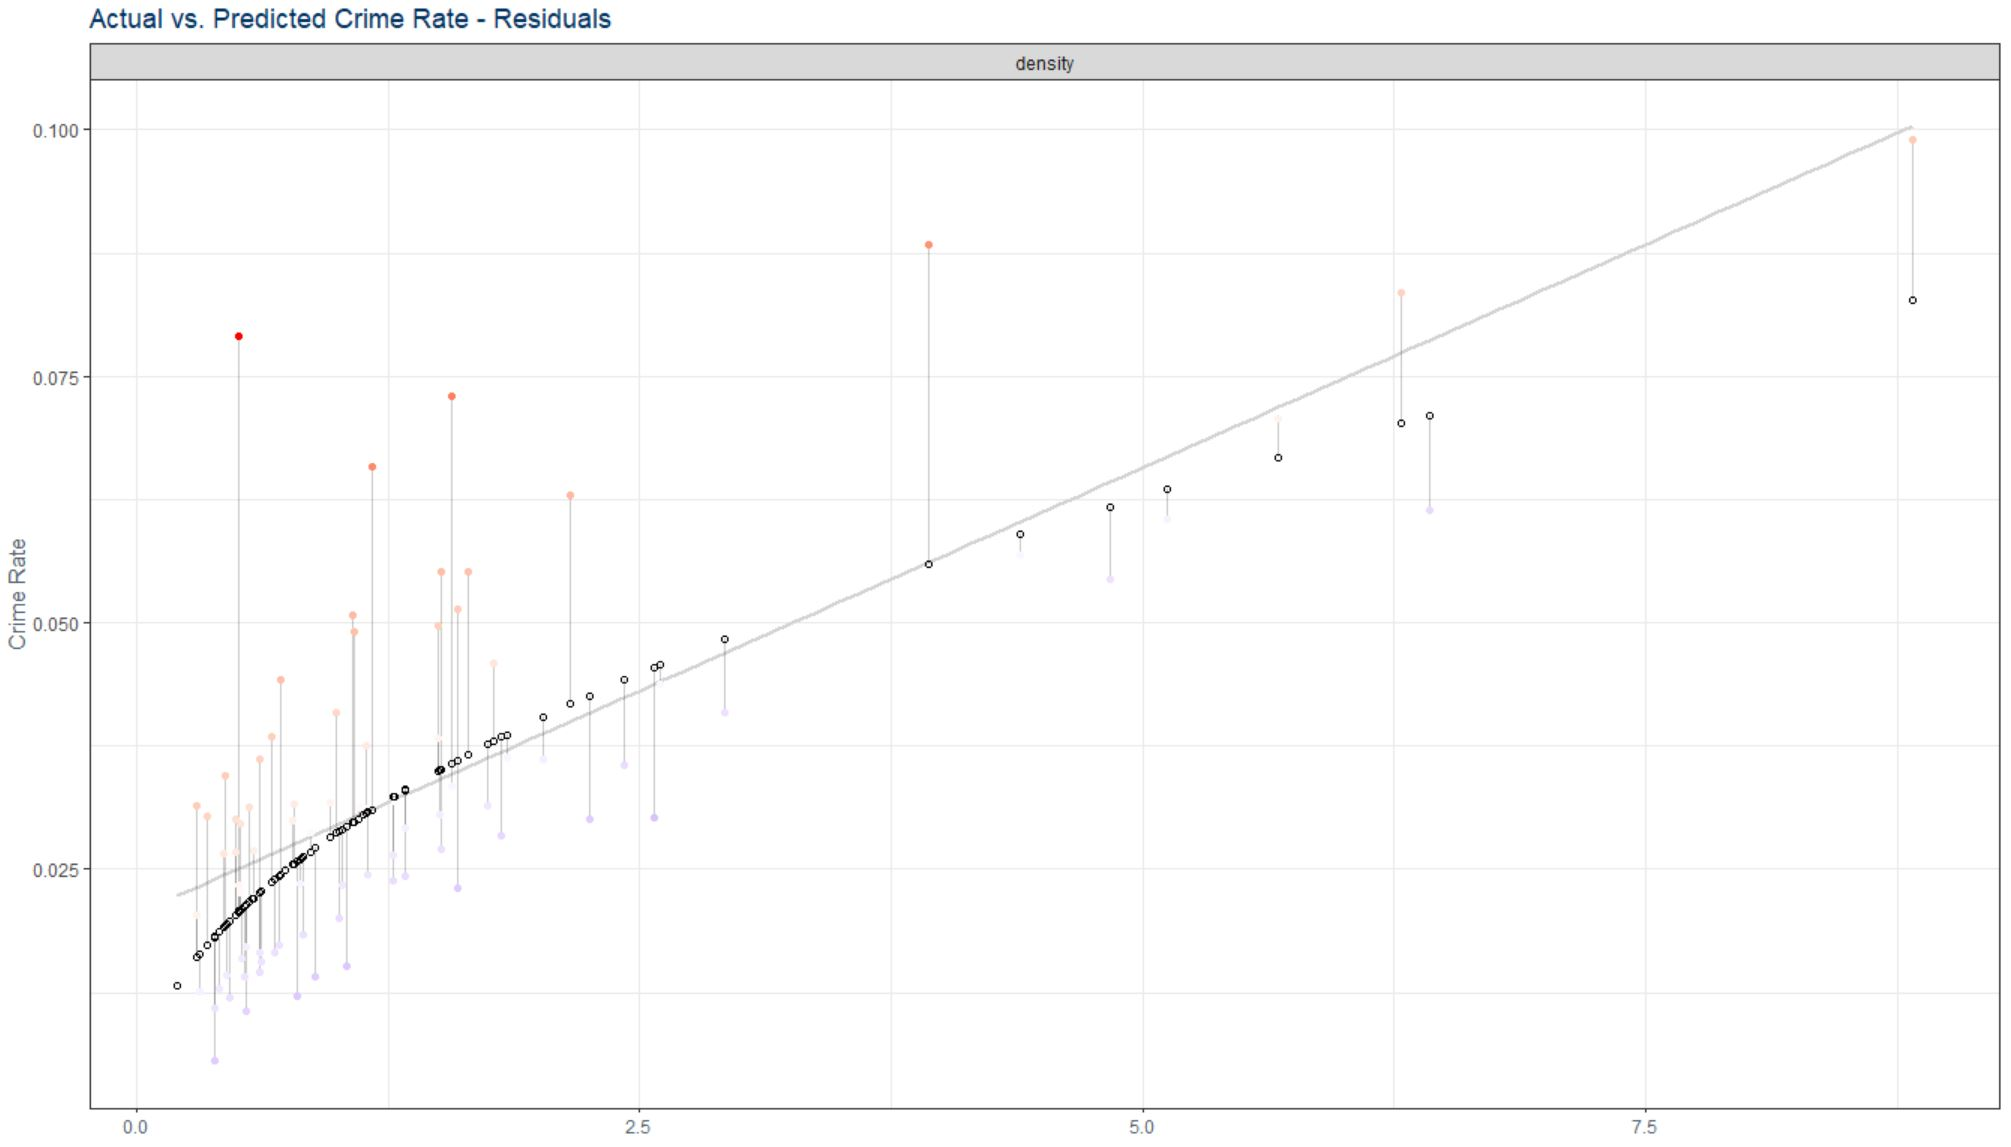
\includegraphics[width=0.9\textwidth]{images/Model_0_residuals.jpg}
	\label{fig:Model0 Residuals}
	\caption{Model : Prediction Error, Naive Model}
\end{figure}

\begin{figure}[!ht]
	\centering
	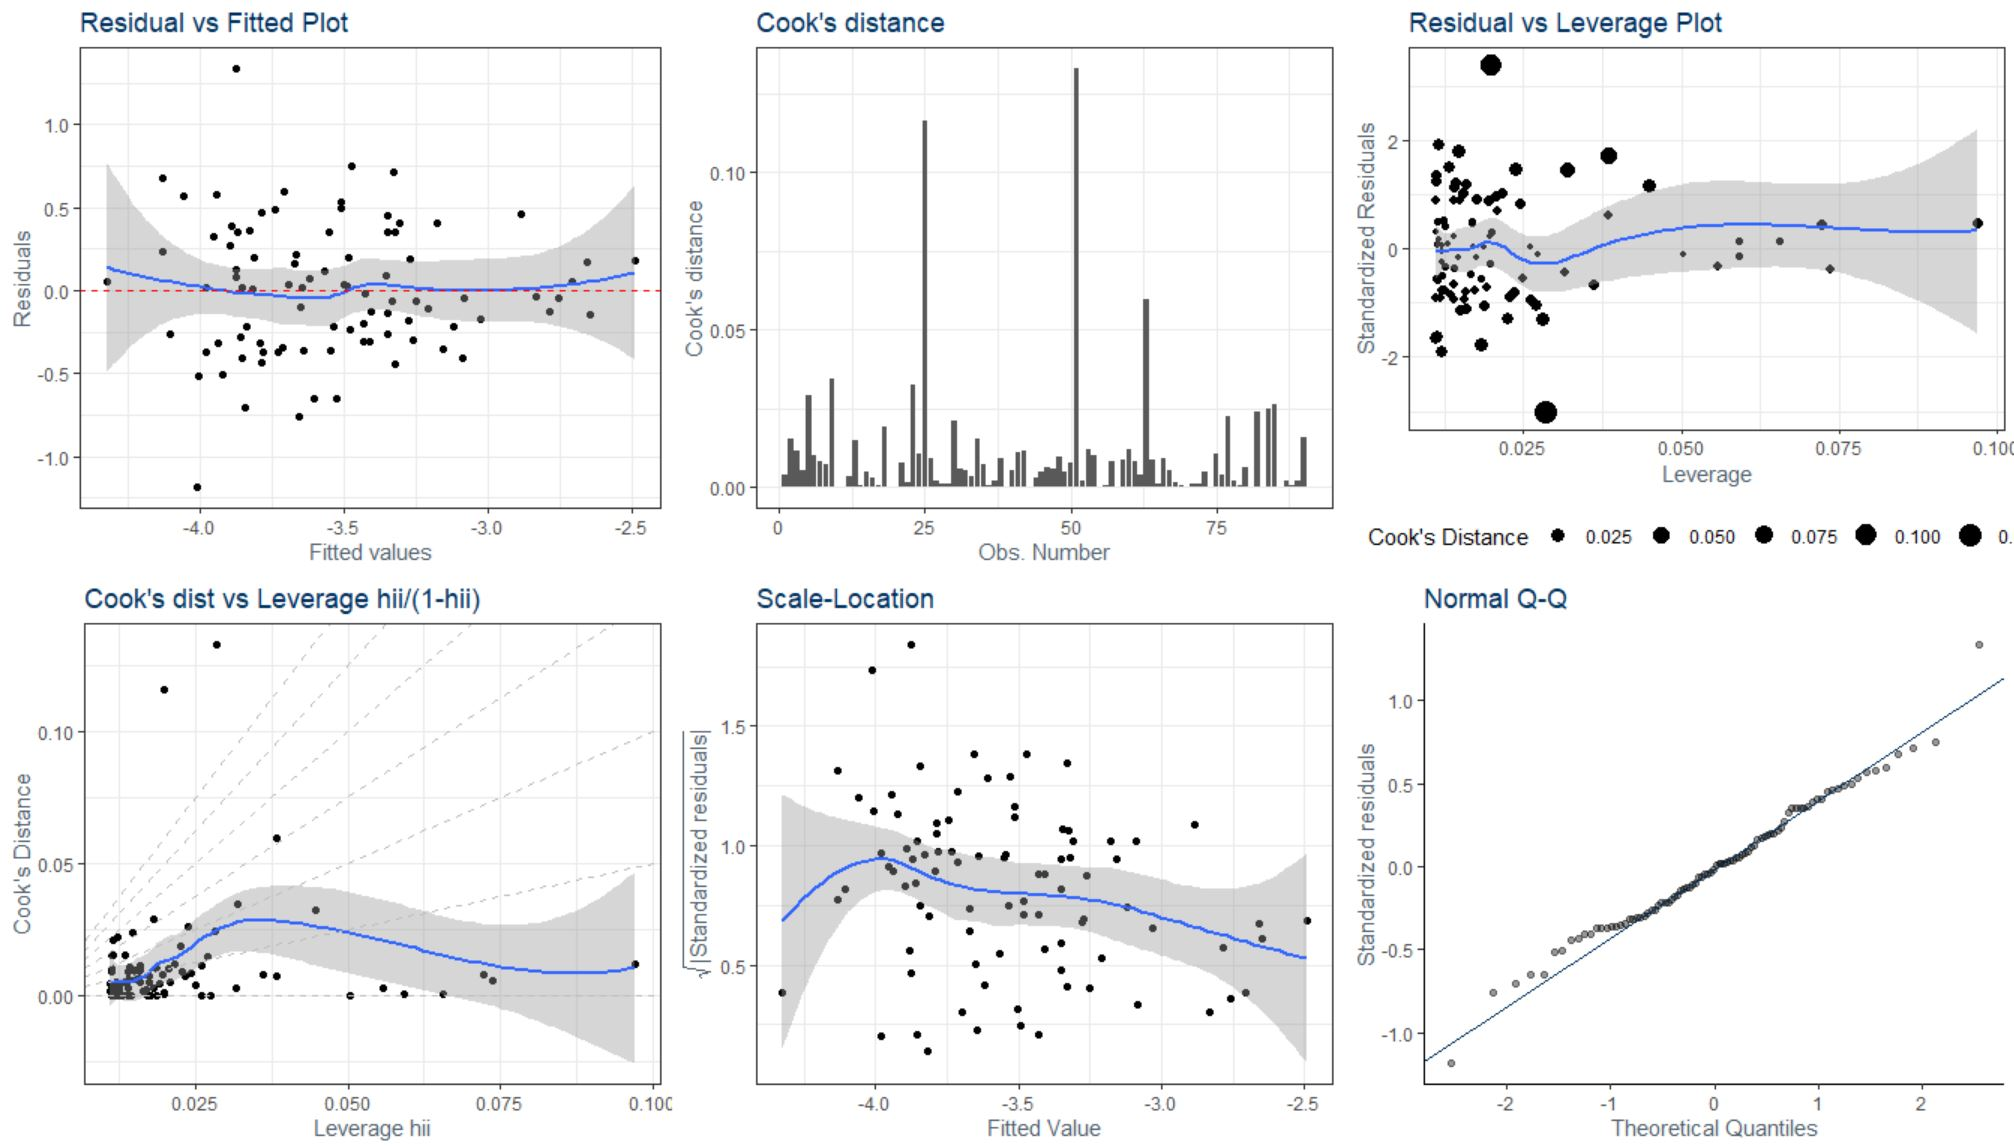
\includegraphics[width=1.0\textwidth]{images/Model_0_diagnostic_plots.jpg}
	\label{fig:Model0 Diagnostic Plots}
	\caption{Model : Diagnostics Plots, Naive Model}
\end{figure}

\pagebreak

\subsection{Manually Tuned Model (Model 1)}

\textit{\textcolor{Grey}{One model with only the explanatory variables of key interest (possibly transformed, as determined by your EDA), and no other covariates.}}\\

Our manually tuned model was built from reasoning through EDA variables and common-sense understanding of the indicators of crime; this resulted in selection of four key variables of interest: $\textcolor{Blue}{log(density)}$, $\textcolor{Blue}{log(pctmin80)}$, $\textcolor{Blue}{prbconv}$, and $\textcolor{Blue}{log(polpc)}$, which resulted in an adjusted $R^2$ of $\textbf{0.760}$:\\

\begin{table}[!htbp] \centering \small
	\caption{Model : Manually Tuned} 
	\begin{tabular}{@{\extracolsep{3pt}}lD{.}{.}{-3} } 
		\\[-1.8ex]\hline 
		\hline \\[-1.8ex] 
		& \multicolumn{1}{c}{\textit{Dependent variable:}} \\ 
		\cline{2-2} 
		\\[-1.8ex] & \multicolumn{1}{c}{\textcolor{Purple}{\textbf{log(crmrte)}}} \\ 
		\hline \\[-1.8ex] 
		\textcolor{Blue}{\textbf{log(density)}} & 0.363^{***}$ $(0.283$, $0.442) \\ 
		\textcolor{Blue}{\textbf{log(pctmin80)}} & 0.226^{***}$ $(0.168$, $0.284) \\ 
		\textcolor{Blue}{\textbf{prbconv}} & -0.433^{***}$ $(-0.596$, $-0.270) \\ 
		\textcolor{Blue}{\textbf{log(polpc)}} & 0.439^{***}$ $(0.249$, $0.628) \\ 
		Constant & -1.126^{*}$ $(-2.357$, $0.104) \\ 
		\hline \\[-1.8ex] 
		Observations & \multicolumn{1}{c}{90} \\ 
		R$^{2}$ & \multicolumn{1}{c}{0.771} \\ 
		Adjusted R$^{2}$ & \multicolumn{1}{c}{0.760} \\ 
		Residual Std. Error & \multicolumn{1}{c}{0.269 (df = 85)} \\ 
		F Statistic & \multicolumn{1}{c}{71.538$^{***}$ (df = 4; 85)} \\ 
		\hline 
		\hline \\[-1.8ex] 
		\textit{Note:}  & \multicolumn{1}{r}{$^{*}$p$<$0.1; $^{**}$p$<$0.05; $^{***}$p$<$0.01} \\ 
	\end{tabular} 
\end{table} 

\begin{table}[!htbp] \centering \small
	\caption{Model : RESET test and Breusch-Pagan test p-values (Manually Tuned)} 
	\label{tbl:BPModel1}
	\begin{tabular}{@{\extracolsep{5pt}} cc} 
		\\[-1.8ex]\hline 
		\hline \\[-1.8ex] 
		RESET (power=2) & Breusch.pagan \\ 
		\hline \\[-1.8ex] 
		$0.346$ & $0.0001$ \\ 
		\hline \\[-1.8ex] 
	\end{tabular} 
\end{table} 

\begin{table}[!htbp] \centering \small
	\caption{Model : VIF Scores (Manually Tuned)} 
	\label{tbl:VIFModel1}
	\begin{tabular}{@{\extracolsep{5pt}} cccc} 
		\\[-1.8ex]\hline 
		\hline \\[-1.8ex] 
		log\_density & log\_pctmin80 & prbconv & log\_polpc \\ 
		\hline \\[-1.8ex] 
		$1.241$ & $1.001$ & $1.065$ & $1.208$ \\ 
		\hline \\[-1.8ex] 
	\end{tabular} 
\end{table} 

\pagebreak

\textbf{\textcolor{OrangeRed}{MODEL 1 - MANUALLY TUNED CONTD.}}\\

\begin{figure}[!ht]
	\centering
	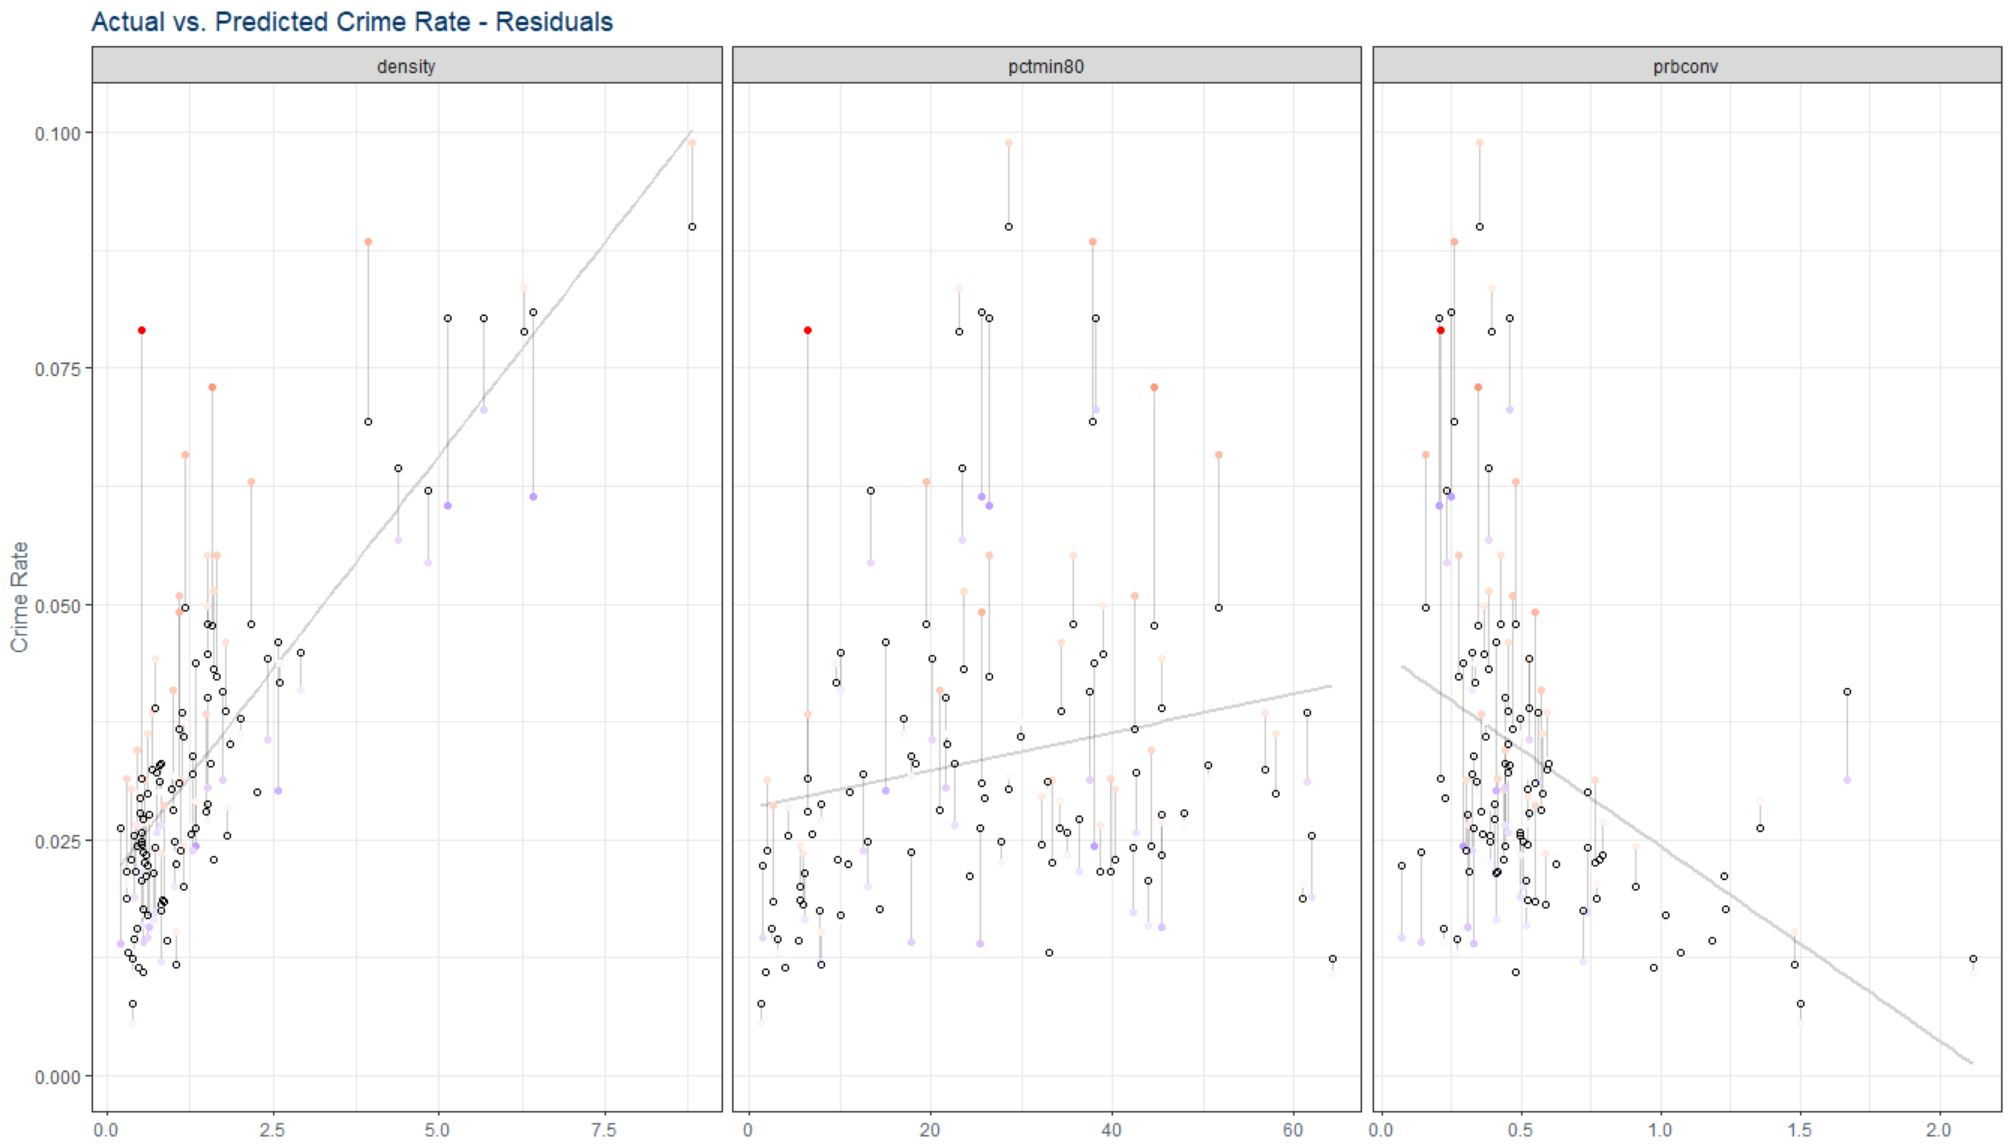
\includegraphics[width=0.95\textwidth]{images/Model_1_residuals.jpg}
	\caption{Model : Prediction Error, Manually Tuned Model}
	\label{fig:Model1 Residuals}
\end{figure}

\begin{figure}[!ht]
	\centering
	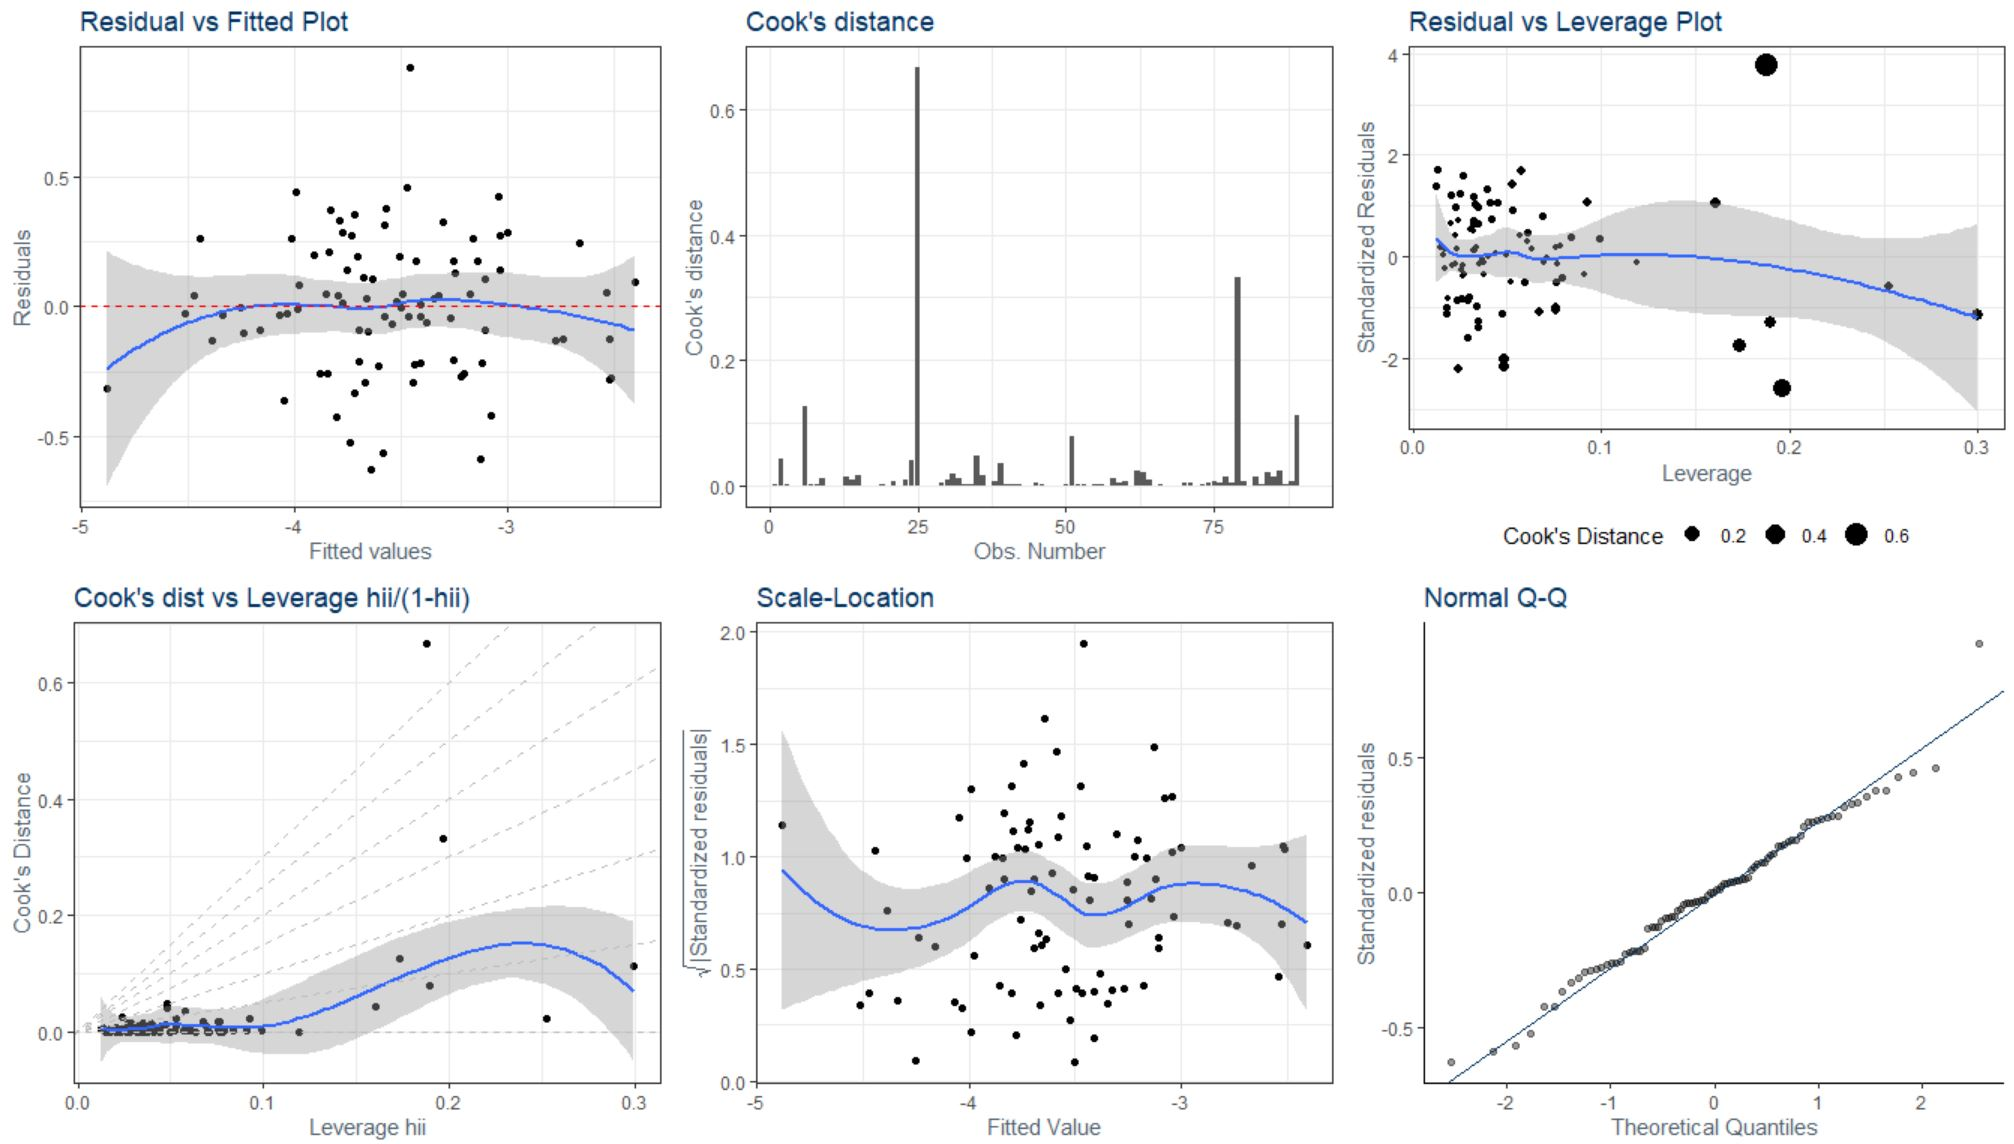
\includegraphics[width=0.95\textwidth]{images/Model_1_diagnostic_plots.jpg}
	\caption{Model : Diagnostic Plots, Manually Tuned Model}
	\label{fig:Model1 Diagnostic Plots}
\end{figure}

\pagebreak

\textbf{\textcolor{OrangeRed}{MODEL 1 - MANUALLY TUNED CONTD.}}\\

Model 1 suggests a strong linear relationship between the density (0.36\%), percent minority (0.27\%), police per capita (0.44\%), and crime rate. There is a negative relationship between probability of conviction and the crime rate (increase probability of conviction by 1 lowers the crime rate by 0.43\%) The model has an R-squared of 77.1\% and adjusted R-squared of 76.0\%. \\

Adding additional variables suggests that there is a less strong relationship between density and the crime rate, which makes sense as there is a medium correlation between the additional variables and there is clear intuition for why each factor impacts the crime rate. Reviewing the residual plots, this model also appears to satisfy all 6 CLM assumptions. There appears to be more heteroscedasticity than in the niave model as the residuals are slightly wider towards the middle than the ends. The Breusch-Pagan test confirms there is heteroscedasticity. We correct for this by using a heteroskedasticity consistent (HC) variance covariance to compute the standard errors. \\

CLM assumption analysis for \textit{MANUALLY TUNED MODEL}:
\label{sec:ManualModelCLM}

\begin{description}[font=$\bullet$~\normalfont\scshape\small\color{red!50!black}]
	\small
	\item [CLM 1 - Linear in parameters] {\fontsize{10}{10} \selectfont : As the linear model is constructed in such a way that that the parameters are linear with error term $u$ , we assess the Linear Assumption as affirmed by definition.}
	\item [CLM 2 - Random sampling] {\fontsize{10}{10} \selectfont : From the \nameref{fig:MissingCountiesGraph} graph in our EDA section, we note that North Carolina has 100 counties, of which we have data for 90; therefore, we have nearly the entire population available for our analysis.  The dispersion of missing counties does not appear to fall along any conceivable pattern, save for a cluster of missing counties near the Eastern border that are geographically connected.  Regardless, we have a sufficient percentage of the population from which we can draw reliable statistical inference and no reason to believe that the sample taken is biased or violates the tenants of IID sampling.}
	\item [CLM 3 - No perfect multi-colinearity] {\fontsize{10}{10} \selectfont : From \nameref{tbl:VIFModel1}, we can review the \href{https://en.wikipedia.org/wiki/Variance_inflation_factor}{Variance inflation factor} scores for each coefficient to evaluate whether there exists a degree of multi-colinearity worth worrying over.  Typically, scores above 4-5 are signal for concern - we see from our results that we do not have significant multi-colinearity in this model.}
	\item [CLM 4 - Zero-conditional mean] {\fontsize{10}{10} \selectfont : To meet this condition, we expect the error term $u$ to be $\approx 0$ for all variables, such that $E(u|x_1,x_2,...,x_n) = 0$.  We can verify this condition by reviewing the \textbf{Residual vs Fitted Plot} (see \ref{fig:Model1 Diagnostic Plots}) and looking for an approximate straight loess line.  Unfortunately, our line is slightly upward-convex, but is being pulled down from the zero-line by only a very few data points.  In order to correct this, we will need to capture more of the variation in the model by adding appropriate variables currently omitted.}
	\item [CLM 5 - Homoskedasticity] {\fontsize{10}{10} \selectfont : Ideally, variance of the error term $u$ in our model remains uniform across all fitted values.  We can assess compliance with this condition via review of the loess line in the \textbf{Scale-Location} plot (see \ref{fig:Model1 Diagnostic Plots}), or by executing a Breusch-pagan test and evaluating the p-values.  From our plot, we see an oscillating pattern for variance, implying that our variance is not sufficiently uniform.  From our BP test (see \ref{tbl:BPModel1}), we receive a p-value of 0.0001 which implies we can easily reject the null hypothesis $H_0 : Homoskedasticity$.}
	\item [CLM 6 - Normality] {\fontsize{10}{10} \selectfont : The assumption here is that the error population is independent [of the regressors] and that the error term $u$ is normally distribution with $\mu = 0$.  We can review this expectation in the \textbf{Normal Q-Q} plot (see \ref{fig:Model1 Diagnostic Plots}); here, we see some slight back-and-forth on the plot, indicating the presence of kurtosis and a possible multi-modal distribution.  In general, our error term is likely non-normally distributed; however, since our sample size is 90 we benefit from asymptotics and the assurance that our coefficients are approximately normal.}
\end{description}

\pagebreak

\subsection{Best Fit Model (Model 2)}
\label{sec:Model2}

\textit{\textcolor{Grey}{One model that includes key explanatory variables and only covariates that you believe increase the accuracy of your results without introducing substantial bias (for example, you should not include outcome variables that will absorb some of the causal effect you are interested in). This model should strike a balance between accuracy and parsimony and reflect your best understanding of the determinants of crime.}}\\

After achieving an $R^2$ of $0.76$ from our best-educated manual selection, we employed the use of \href{https://www.rdocumentation.org/packages/leaps/versions/2.1-1/topics/regsubsets}{regSubsets} to assist in feature selection that would perform well and avoid over-fitting.  Our resulting model incorporated eight of the input features, including a mix of native and log-transformed values, and achieved an adjusted $R^2$ of $\textbf{0.855}$:\\


\begin{table}[!htbp] \centering \small
	\caption{Model : Best Fit} 
	\begin{tabular}{@{\extracolsep{3pt}}lD{.}{.}{-3} } 
		\\[-1.8ex]\hline 
		\hline \\[-1.8ex] 
		& \multicolumn{1}{c}{\textit{Dependent variable:}} \\ 
		\cline{2-2} 
		\\[-1.8ex] & \multicolumn{1}{c}{\textcolor{Purple}{\textbf{log(crmrte)}}} \\ 
		\hline \\[-1.8ex] 
		\textcolor{Blue}{\textbf{prbconv}} & -1.053^{***}$ $(-1.339$, $-0.766) \\ 
		\textcolor{Blue}{\textbf{pctmin80}} & 0.014^{***}$ $(0.011$, $0.016) \\ 
		\textcolor{Blue}{\textbf{wfir}} & -0.001^{**}$ $(-0.002$, $-0.0002) \\ 
		\textcolor{Blue}{\textbf{log(prbarr)}} & -0.426^{***}$ $(-0.541$, $-0.311) \\ 
		\textcolor{Blue}{\textbf{log(polpc)}} & 0.464^{***}$ $(0.307$, $0.621) \\ 
		\textcolor{Blue}{\textbf{log(density)}} & 0.363^{***}$ $(0.290$, $0.436) \\ 
		\textcolor{Blue}{\textbf{log(taxpc)}} & -1.322^{***}$ $(-1.901$, $-0.743) \\ 
		\textcolor{Blue}{\textbf{log(wsta)}} & -0.397^{**}$ $(-0.742$, $-0.052) \\ 
		Constant & 5.698^{***}$ $(2.803$, $8.594) \\ 
		\hline \\[-1.8ex] 
		Observations & \multicolumn{1}{c}{90} \\ 
		R$^{2}$ & \multicolumn{1}{c}{0.869} \\ 
		Adjusted R$^{2}$ & \multicolumn{1}{c}{0.855} \\ 
		Residual Std. Error & \multicolumn{1}{c}{0.184 (df = 79)} \\ 
		F Statistic & \multicolumn{1}{c}{71.006$^{***}$ (df = 10; 79)} \\ 
		\hline 
		\hline \\[-1.8ex] 
		\textit{Note:}  & \multicolumn{1}{r}{$^{*}$p$<$0.1; $^{**}$p$<$0.05; $^{***}$p$<$0.01} \\ 
	\end{tabular} 
\end{table} 

\begin{table}[!htbp] \centering \small
	\caption{Model : RESET test and Breusch-Pagan test p-values (Best Fit)} 
	\label{tbl:BPModel2}
	\begin{tabular}{@{\extracolsep{5pt}} cc} 
		\\[-1.8ex]\hline 
		\hline \\[-1.8ex] 
		RESET (power=2) & Breusch-pagan \\ 
		\hline \\[-1.8ex] 
		$0.00004$ & $0.00002$ \\ 
		\hline \\[-1.8ex] 
	\end{tabular} 
\end{table} 

\begin{table}[!htbp] \centering \small
	\caption{Model : VIF Scores (Best Fit)} 
	\label{tbl:VIFModel2}
	\begin{tabular}{@{\extracolsep{5pt}} cccccccc} 
		\\[-1.8ex]\hline 
		\hline \\[-1.8ex] 
		prbconv & pctmin80 & wfir & log\_prbarr & log\_polpc & log\_density & log\_taxpc & log\_wsta \\ 
		\hline \\[-1.8ex] 
		$1.318$ & $1.070$ & $1.654$ & $1.426$ & $1.570$ & $2.176$ & $1.392$ & $1.182$ \\ 
		\hline \\[-1.8ex] 
	\end{tabular} 
\end{table} 

\pagebreak

\textbf{\textcolor{OrangeRed}{MODEL 2 - BEST FIT CONTD.}}\\

Our feature selection algorithm selection was made using the lowest BIC score, which had a slightly lower overall $R^2$ value, but provides us with a more robust model:

\begin{figure}[!ht]
	\begin{subfigure}[b]{0.5\textwidth}
		\centering
		\caption{Input Features by BIC score}
		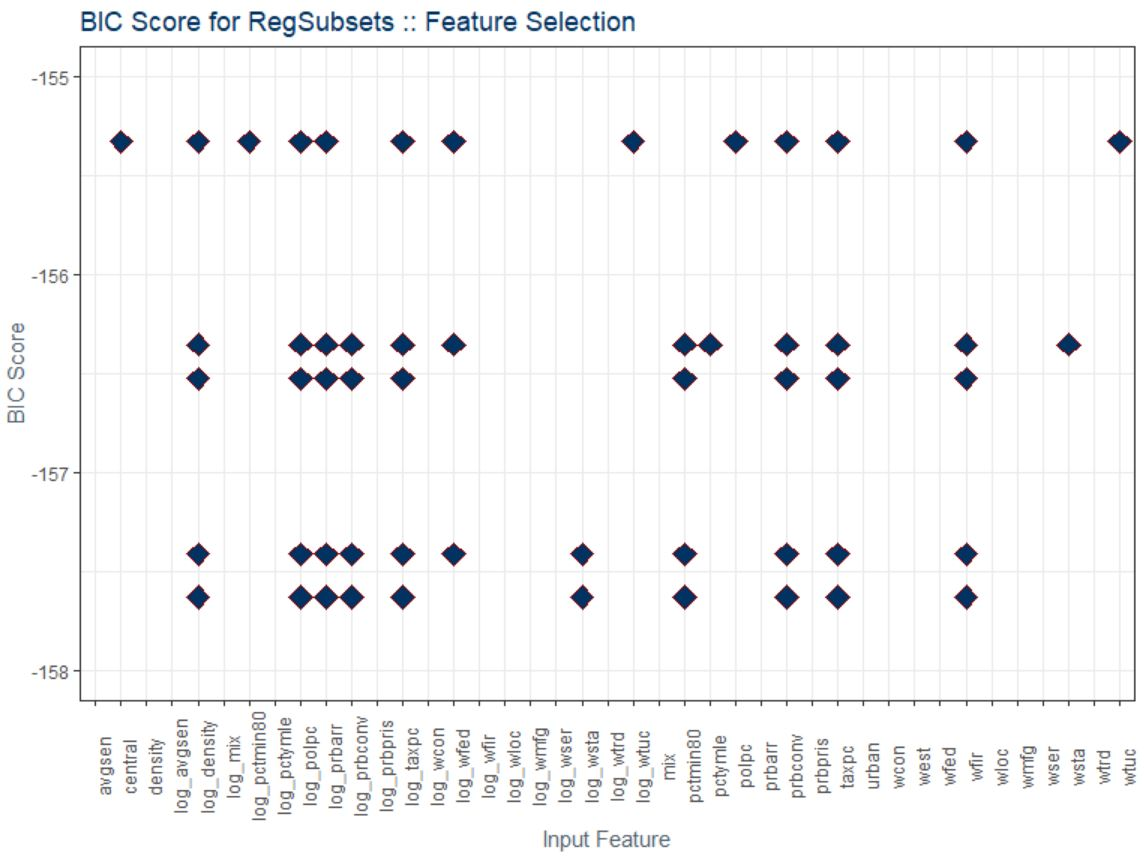
\includegraphics[width=\linewidth]{images/Model_2_feature_selection_bic.jpg}
		\label{fig:Model2 Feature Selection BIC scores}
	\end{subfigure}\vspace{3mm}% or \hspace{0.3\textwidth}
	\hfill
	\begin{subfigure}[b]{0.5\textwidth}
		\centering
		\caption{Adjusted R-Squared by BIC score}
		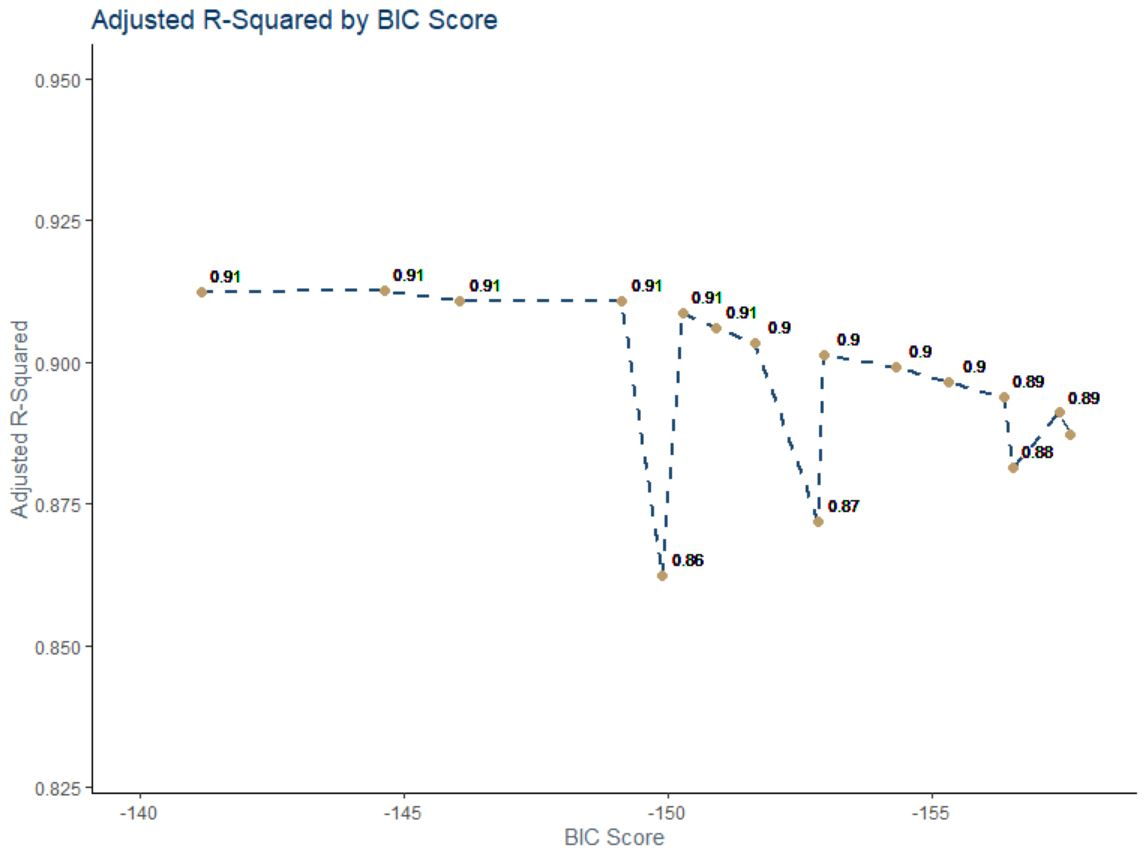
\includegraphics[width=\linewidth]{images/Model_2_feature_selection_adjr2.jpg}
		\label{fig:Model2 Adjusted R-Squared by BIC}
	\end{subfigure}
	\label{fig:Model2 Feature Selection}
	\caption{Model : Feature Selection, Best Fit Model}
\end{figure}

\begin{figure}[!ht]
	\centering
	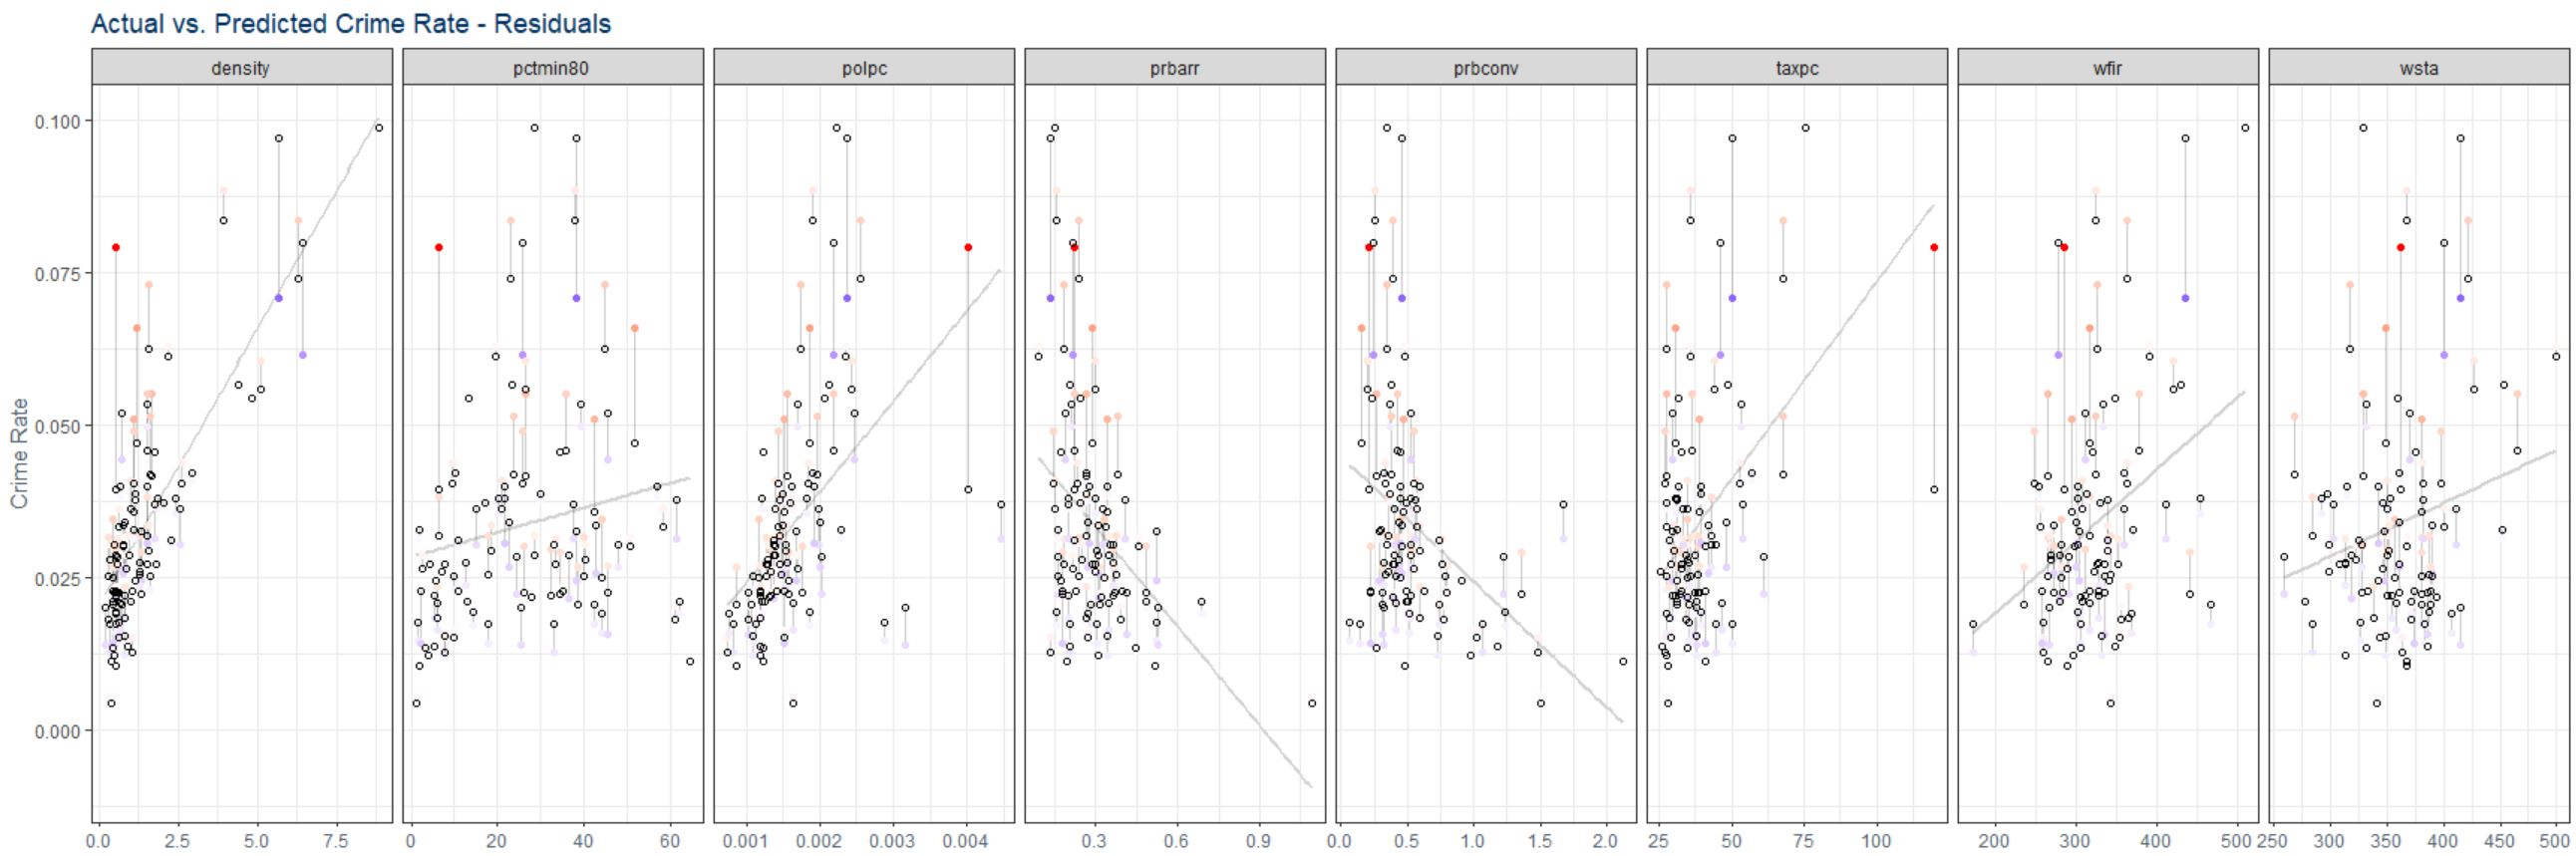
\includegraphics[width=1.00\textwidth]{images/Model_2_residuals.jpg}
	\label{fig:Model2 Residuals}
	\caption{Model : Prediction Error, Best Fit Model}
\end{figure}

\pagebreak

\textbf{\textcolor{OrangeRed}{MODEL 2 - BEST FIT CONTD.}}\\

\begin{figure}[!ht]
	\centering
	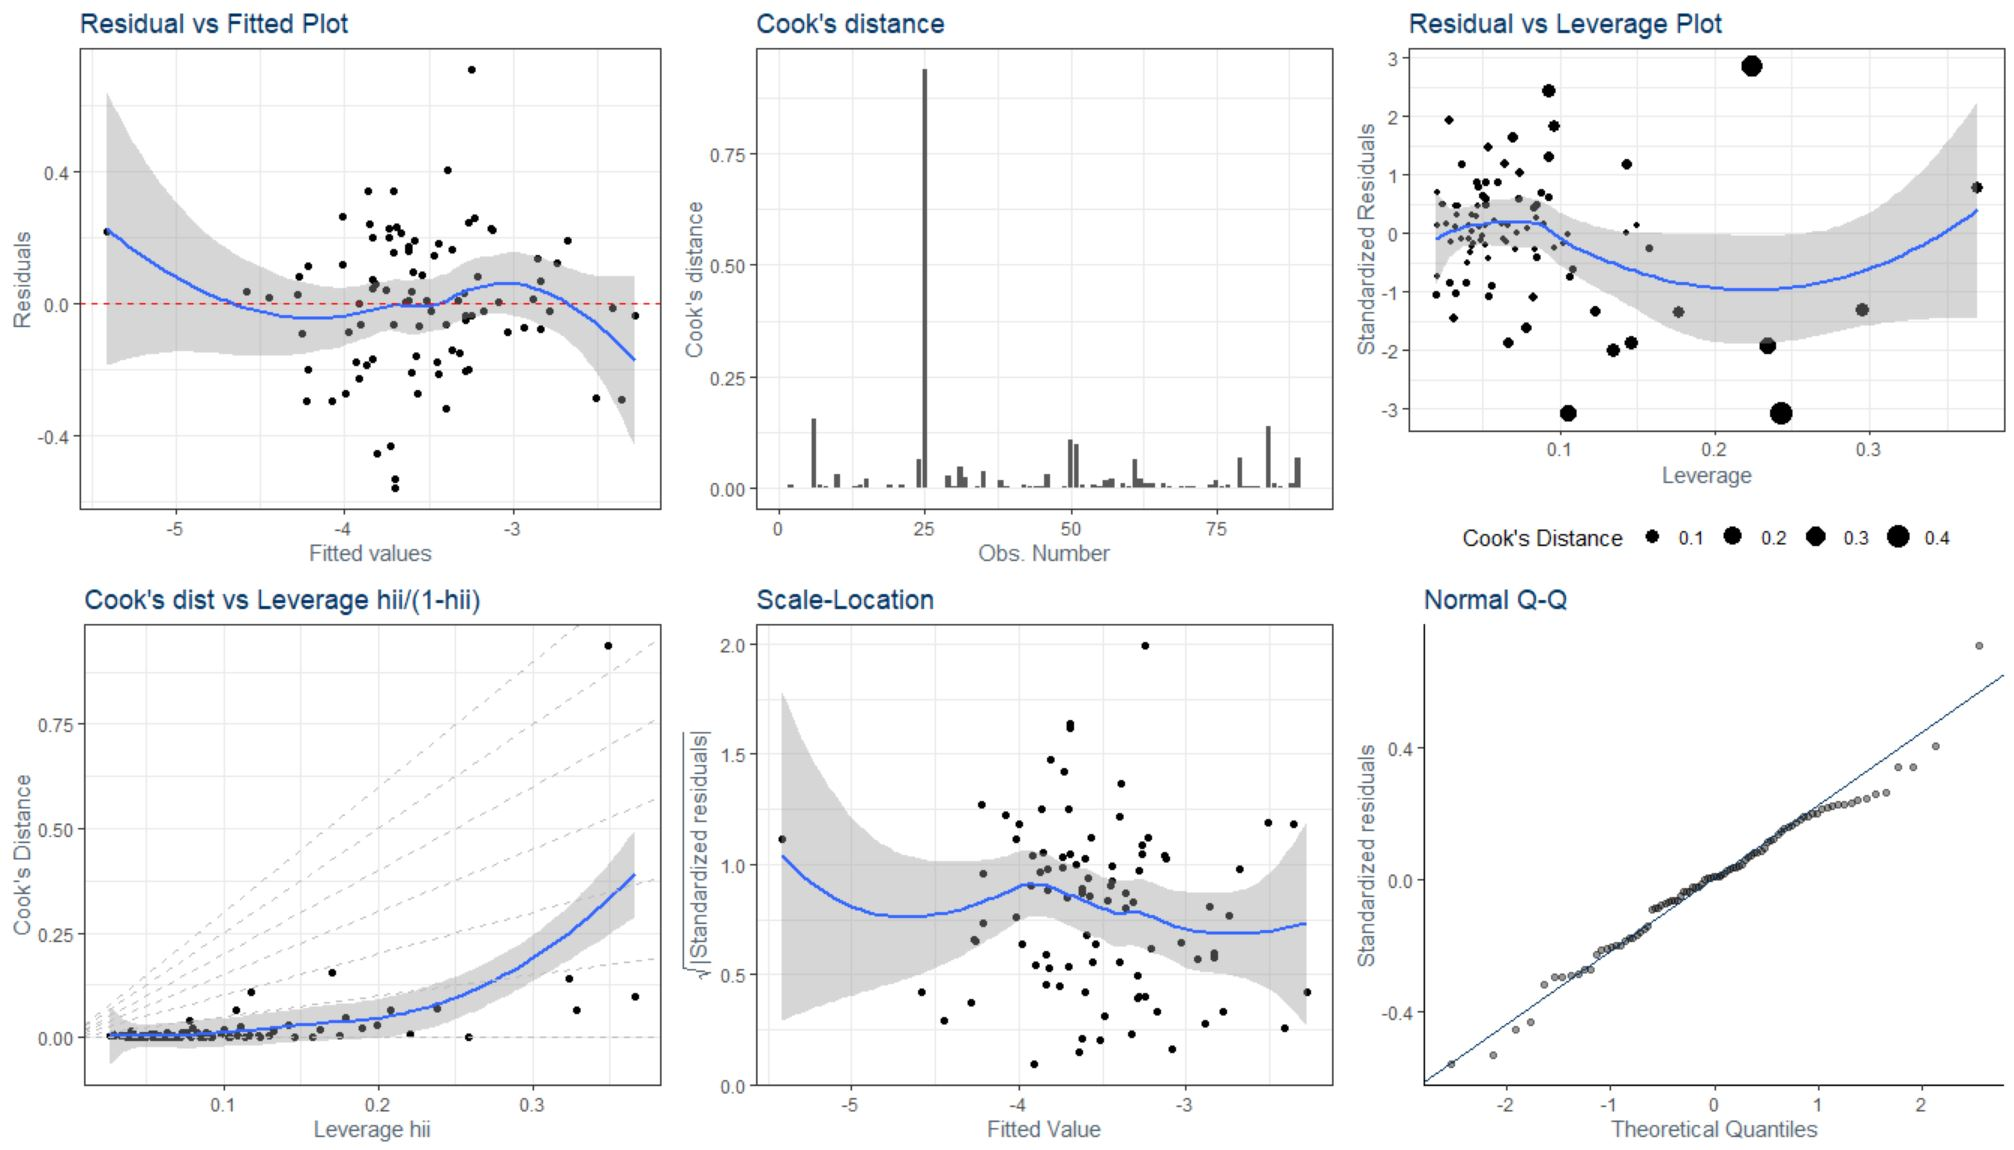
\includegraphics[width=0.95\textwidth]{images/Model_2_diagnostic_plots.jpg}
	\caption{Model : Diagnostic Plots, Best Fit Model}
	\label{fig:Model2 Diagnostic Plots}
\end{figure}

\begin{figure}[!ht]
	\centering
	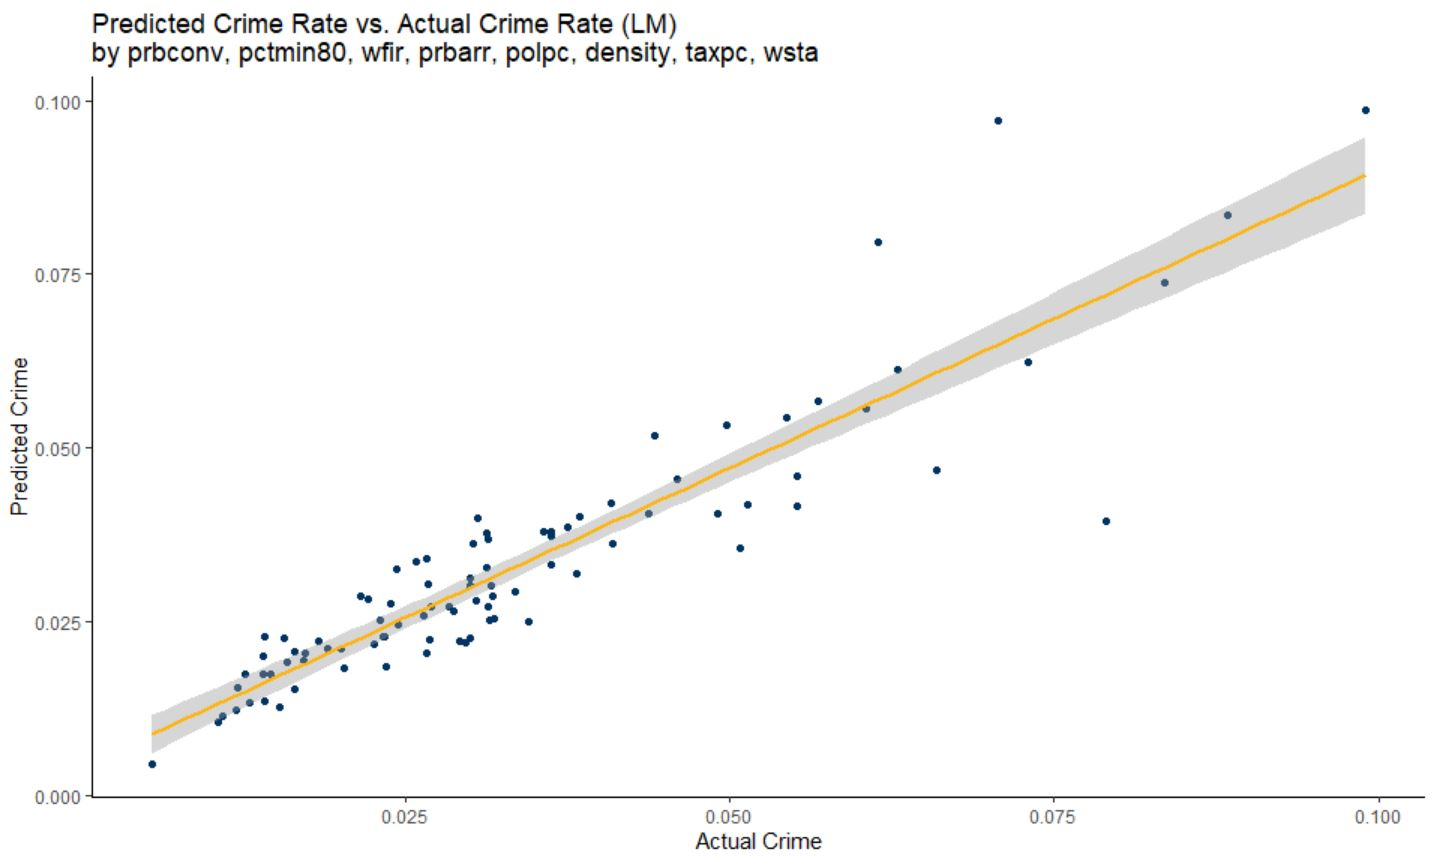
\includegraphics[width=0.95\textwidth]{images/Model_2_performance.jpg}
	\caption{Model : Predicted vs. Actual, Best Fit Model}
	\label{fig:Model2 Performance}
\end{figure}

\pagebreak

\textbf{\textcolor{OrangeRed}{MODEL 2 - BEST FIT CONTD.}}\\

CLM assumption analysis for \textit{BEST-FIT MODEL}:
\label{sec:BestFitModelCLM}

\begin{description}[font=$\bullet$~\normalfont\scshape\small\color{red!50!black}]
	\item [CLM 1 - Linear in parameters] {\fontsize{10}{10} \selectfont : \textit{Same as CLM 1 for Manually Tuned Model (see \nameref{sec:ManualModelCLM})}.}
	\item [CLM 2 - Random sampling] {\fontsize{10}{10} \selectfont : \textit{Same as CLM 2 for Manually Tuned Model (see \nameref{sec:ManualModelCLM})}.}
	\item [CLM 3 - No perfect multi-colinearity] {\fontsize{10}{10} \selectfont : From \nameref{tbl:VIFModel2}, we can review the \href{https://en.wikipedia.org/wiki/Variance_inflation_factor}{Variance inflation factor} scores for each coefficient to evaluate whether there exists a degree of multi-colinearity worth worrying over.  Typically, scores above 4-5 are signal for concern - we see from our results that we do not have significant multi-colinearity in this model.}
	\item [CLM 4 - Zero-conditional mean] {\fontsize{10}{10} \selectfont : To meet this condition, we expect the error term $u$ to be $\approx 0$ for all variables, such that $E(u|x_1,x_2,...,x_n) = 0$.  We can verify this condition by reviewing the \textbf{Residual vs Fitted Plot} (see \ref{fig:Model2 Diagnostic Plots}) and looking for an approximate straight loess line.  Unfortunately, our line is S-curved, but is being pulled away from the zero-line by only a very few data points.  In order to correct this, we will need to capture more of the variation in the model by adding appropriate variables currently omitted and, potentially, eliminate one or more noise variables.}
	\item [CLM 5 - Homoskedasticity] {\fontsize{10}{10} \selectfont : Ideally, variance of the error term $u$ in our model remains uniform across all fitted values.  We can assess compliance with this condition via review of the loess line in the \textbf{Scale-Location} plot (see \ref{fig:Model2 Diagnostic Plots}), or by executing a Breusch-pagan test and evaluating the p-values.  From our plot, we see an oscillating pattern for variance, implying that our variance is not sufficiently uniform.  From our BP test (see \ref{tbl:BPModel2}), we receive a p-value of 0.00002 which implies we can easily reject the null hypothesis $H_0 : Homoskedasticity$.}
	\item [CLM 6 - Normality] {\fontsize{10}{10} \selectfont : The assumption here is that the error population is independent [of the regressors] and that the error term $u$ is normally distribution with $\mu = 0$.  We can review this expectation in the \textbf{Normal Q-Q} plot (see \ref{fig:Model2 Diagnostic Plots}); here, we see some slight back-and-forth on the plot, indicating the presence of kurtosis and a possible multi-modal distribution.  In general, our error term is likely non-normally distributed; however, since our sample size is 90 we benefit from asymptotics and the assurance that our coefficients are approximately normal.}
\end{description}

\pagebreak

\subsection{Overfit Model (Model 3)}
\label{sec:Model3}

\textit{\textcolor{Grey}{One model that includes the previous covariates, and most, if not all, other covariates. A key purpose of this model is to demonstrate the robustness of your results to model specification.}}\\

For our final model, we ask \href{https://www.rdocumentation.org/packages/MASS/versions/7.3-51.4/topics/stepAIC}{stepAIC} to consider all input parameters, including those that are perfectly multi-colinear, and generate the best performing model.  Here, we achieve a deceiving adjusted $R^2$ of $\textbf{0.913}$ but critical CLM assumptions are likely violated in the process.\\


\begin{table}[!htbp] \centering \small
	\caption{Model : Overfit} 
	\label{} 
	\begin{tabular}{@{\extracolsep{3pt}}lD{.}{.}{-3} } 
		\\[-1.8ex]\hline 
		\hline \\[-1.8ex] 
		& \multicolumn{1}{c}{\textit{Dependent variable:}} \\ 
		\cline{2-2} 
		\\[-1.8ex] & \multicolumn{1}{c}{\textcolor{Purple}{\textbf{log(crmrte)}}} \\ 
		\hline \\[-1.8ex] 
		\textcolor{Blue}{\textbf{prbconv}} & -0.786^{***}$ $(-1.086$, $-0.487) \\ 
		\textcolor{Blue}{\textbf{polpc}} & -344.709^{**}$ $(-619.648$, $-69.770) \\ 
		\textcolor{Blue}{\textbf{taxpc}} & 0.027^{***}$ $(0.015$, $0.040) \\ 
		\textcolor{Blue}{\textbf{central}} & -0.135^{***}$ $(-0.219$, $-0.051) \\ 
		\textcolor{Blue}{\textbf{pctmin80}} & 0.007^{**}$ $(0.001$, $0.013) \\ 
		\textcolor{Blue}{\textbf{wtuc}} & -0.003^{**}$ $(-0.005$, $-0.001) \\ 
		\textcolor{Blue}{\textbf{wfir}} & -0.001^{***}$ $(-0.002$, $-0.0004) \\ 
		\textcolor{Blue}{\textbf{wser}} & 0.009^{**}$ $(0.001$, $0.017) \\ 
		\textcolor{Blue}{\textbf{wmfg}} & -0.004^{***}$ $(-0.006$, $-0.001) \\ 
		\textcolor{Blue}{\textbf{log(prbarr)}} & -0.419^{***}$ $(-0.529$, $-0.309) \\ 
		\textcolor{Blue}{\textbf{log(prbconv)}} & 0.181^{*}$ $(-0.013$, $0.375) \\ 
		\textcolor{Blue}{\textbf{log(polpc)}} & 1.089^{***}$ $(0.573$, $1.606) \\ 
		\textcolor{Blue}{\textbf{log(density)}} & 0.310^{***}$ $(0.233$, $0.387) \\ 
		\textcolor{Blue}{\textbf{log(taxpc)}} & -1.195^{***}$ $(-1.800$, $-0.591) \\ 
		\textcolor{Blue}{\textbf{log(pctmin80)}} & 0.111^{*}$ $(-0.007$, $0.228) \\ 
		\textcolor{Blue}{\textbf{log(wcon)}} & 0.280^{*}$ $(-0.008$, $0.567) \\ 
		\textcolor{Blue}{\textbf{log(wtuc)}} & 1.161^{**}$ $(0.228$, $2.094) \\ 
		\textcolor{Blue}{\textbf{log(wser)}} & -2.715^{***}$ $(-4.690$, $-0.739) \\ 
		\textcolor{Blue}{\textbf{log(wmfg)}} & 1.421^{***}$ $(0.483$, $2.359) \\ 
		\textcolor{Blue}{\textbf{log(wsta)}} & -0.348^{*}$ $(-0.690$, $-0.006) \\ 
		\textcolor{Blue}{\textbf{log(wloc)}} & 0.479^{*}$ $(-0.072$, $1.029) \\ 
		Constant & 4.905$ $(-5.987$, $15.796) \\ 
		\hline \\[-1.8ex] 
		Observations & \multicolumn{1}{c}{90} \\ 
		R$^{2}$ & \multicolumn{1}{c}{0.933} \\ 
		Adjusted R$^{2}$ & \multicolumn{1}{c}{0.913} \\ 
		Residual Std. Error & \multicolumn{1}{c}{0.162 (df = 68)} \\ 
		F Statistic & \multicolumn{1}{c}{45.280$^{***}$ (df = 21; 68)} \\ 
		\hline 
		\hline \\[-1.8ex] 
		\textit{Note:}  & \multicolumn{1}{r}{$^{*}$p$<$0.1; $^{**}$p$<$0.05; $^{***}$p$<$0.01} \\ 
	\end{tabular} 
\end{table} 

\pagebreak

\textbf{\textcolor{OrangeRed}{MODEL 3 - OVERFIT CONTD.}}\\

\begin{table}[!htbp] \centering \small
	\caption{Model : RESET test and Breusch-Pagan test p-values (Overfit)} 
	\label{sec:BPModel3}
	\begin{tabular}{@{\extracolsep{5pt}} cc} 
		\\[-1.8ex]\hline 
		\hline \\[-1.8ex] 
		RESET (power=2) & Breusch.pagan \\ 
		\hline \\[-1.8ex] 
		$0.942$ & $0.800$ \\ 
		\hline \\[-1.8ex] 
	\end{tabular} 
\end{table} 

\begin{table}[!htbp] \centering \small
	\caption{Model : VIF Scores (Overfit)} 
	\label{sec:VIFModel3}
	\begin{tabular}{@{\extracolsep{5pt}} ccccccc} 
		\\[-1.8ex]\hline 
		\hline \\[-1.8ex] 
		prbconv & polpc & taxpc & central & pctmin80 & wtuc & wfir \\ 
		\hline \\[-1.8ex] 
		$9.899$ & $24.550$ & $22.879$ & $1.489$ & $10.560$ & $31.481$ & $2.409$ \\ 
		\hline \\[-1.8ex] 
	\end{tabular} 
\end{table} 

\begin{table}[!htbp] \centering \small
	\caption{Model : VIF Scores Contd. 1/2 (Overfit)}
	\begin{tabular}{@{\extracolsep{5pt}} ccccccc} 
		\\[-1.8ex]\hline 
		\hline \\[-1.8ex] 
		wser & wmfg & log\_prbarr & log\_prbconv & log\_polpc & log\_density & log\_taxpc \\ 
		\hline \\[-1.8ex] 
		$108.478$ & $43.072$ & $1.731$ & $10.309$ & $24.688$ & $3.182$ & $22.632$ \\ 
		\hline \\[-1.8ex] 
	\end{tabular} 
\end{table} 

\begin{table}[!htbp] \centering \small
	\caption{Model : VIF Scores Contd. 2/2 (Overfit)}
	\begin{tabular}{@{\extracolsep{5pt}} ccccccc} 
		\\[-1.8ex]\hline 
		\hline \\[-1.8ex] 
		log\_pctmin80 & log\_wcon & log\_wtuc & log\_wser & log\_wmfg & log\_wsta & log\_wloc \\ 
		\hline \\[-1.8ex] 
		$11.199$ & $1.960$ & $31.227$ & $107.342$ & $45.781$ & $1.506$ & $2.161$ \\ 
		\hline \\[-1.8ex] 
	\end{tabular} 
\end{table} 

\pagebreak

\textbf{\textcolor{OrangeRed}{MODEL 3 - OVERFIT CONTD.}}\\

\begin{figure}[!ht]
	\centering
	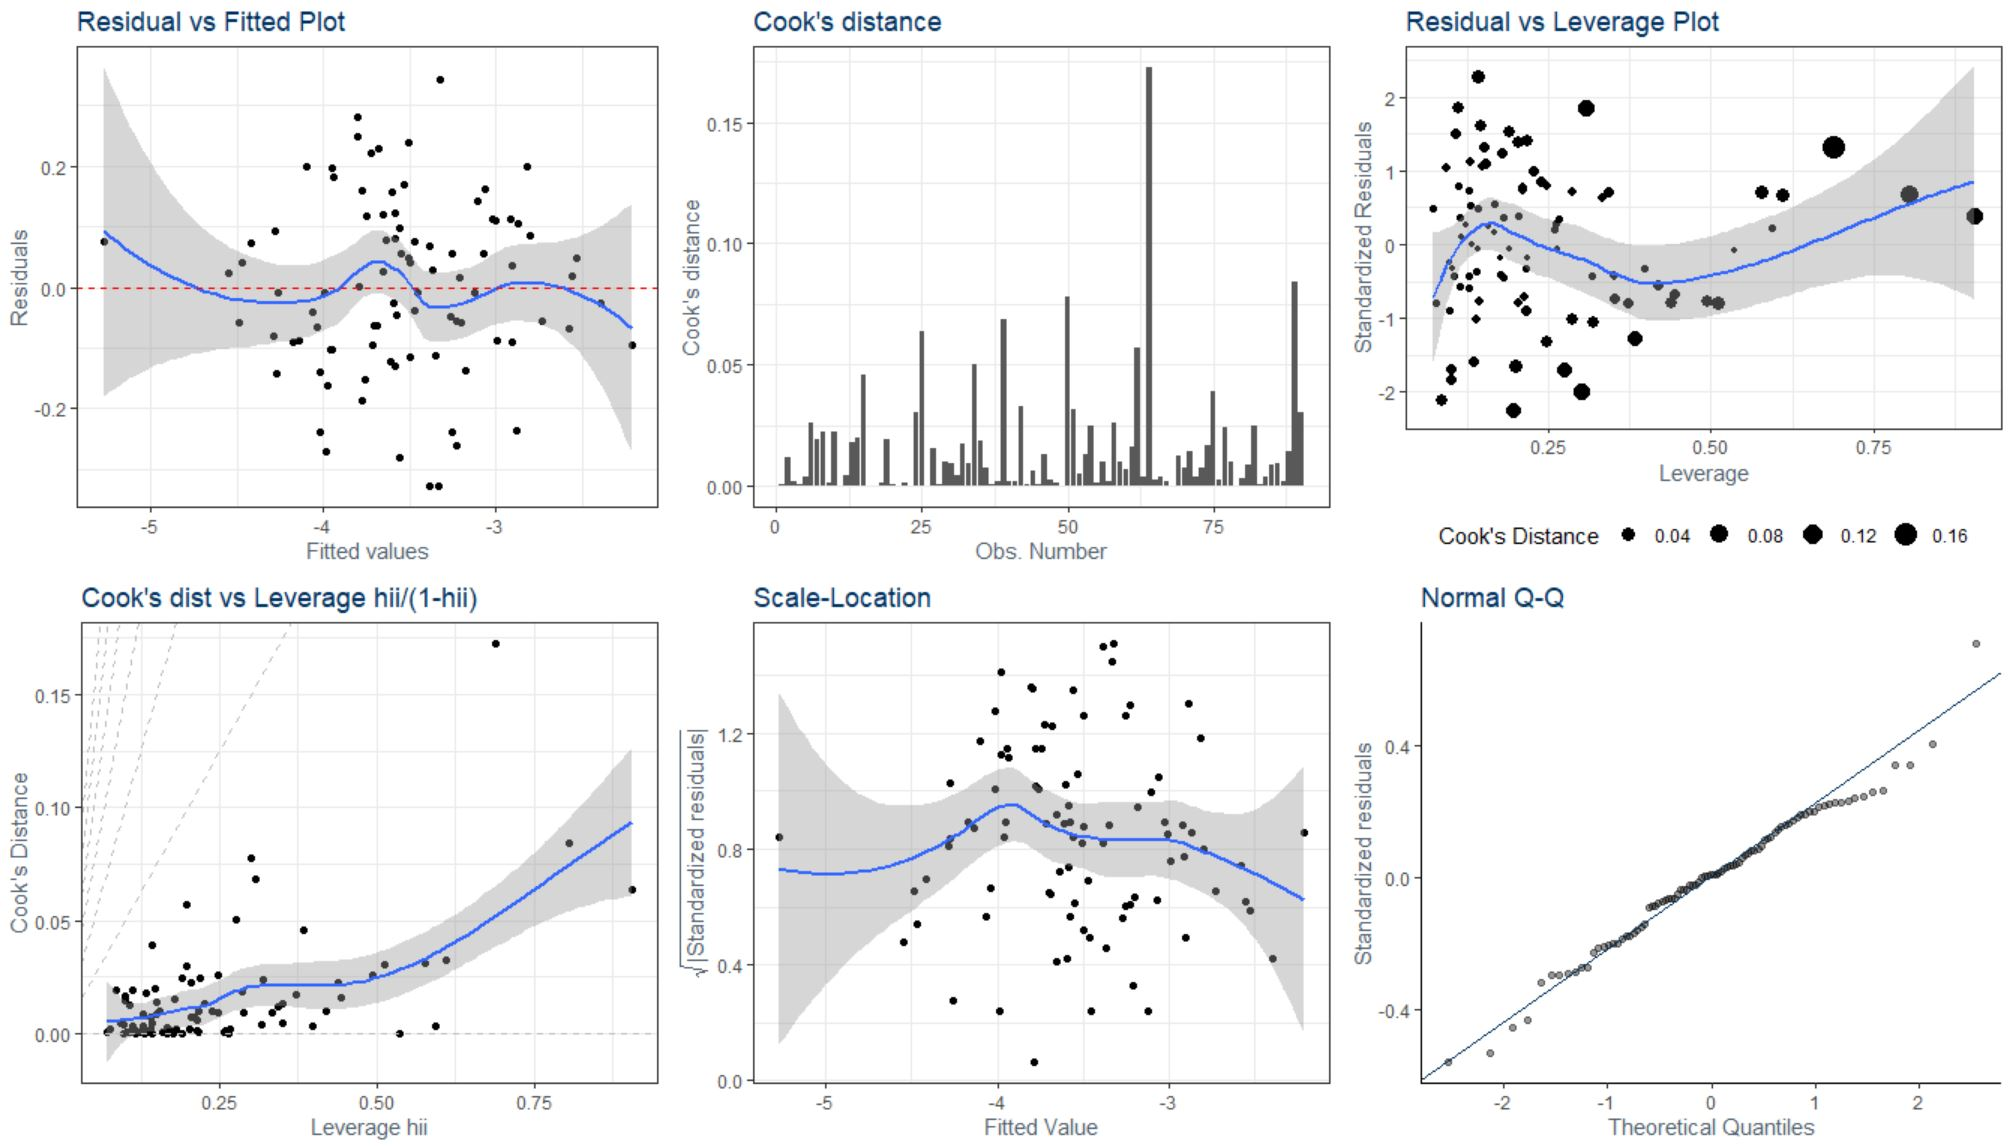
\includegraphics[width=0.95\textwidth]{images/Model_3_diagnostic_plots.jpg}
	\caption{Model : Diagnostic Plots, Overfit Model}
	\label{fig:Model3 Diagnostic Plots}
\end{figure}

\begin{figure}[!ht]
	\centering
	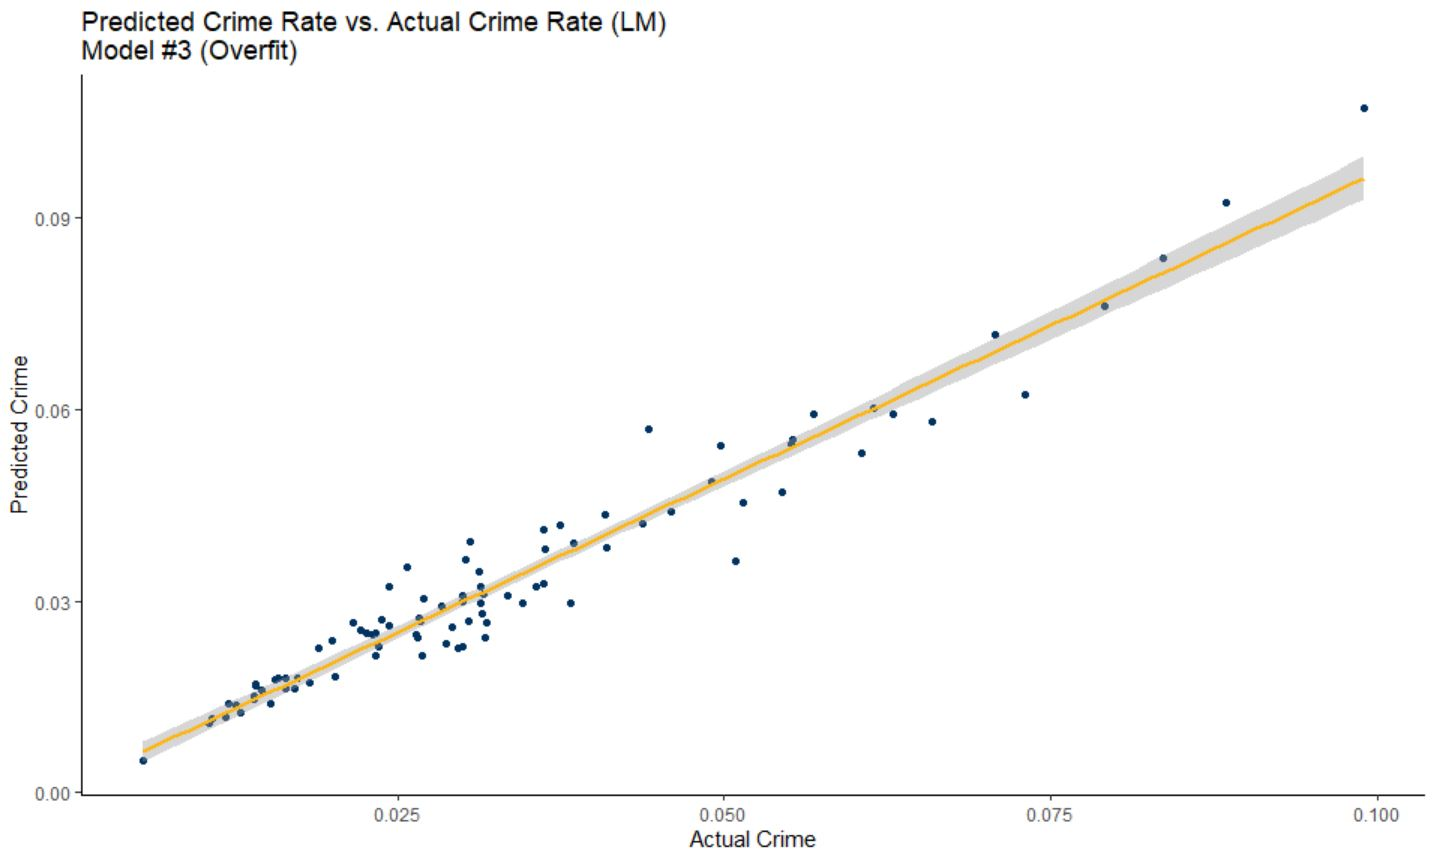
\includegraphics[width=0.8\textwidth]{images/Model_3_performance.jpg}
	\caption{Model : Predicted vs. Actual, Overfit Model}
	\label{fig:Model3 Performance}
\end{figure}

\pagebreak

\textbf{\textcolor{OrangeRed}{MODEL 3 - OVERFIT CONTD.}}\\

CLM assumption analysis for \textit{OVERFIT MODEL}:\\
\label{sec:OverfitModelCLM}

\begin{description}[font=$\bullet$~\normalfont\scshape\small\color{red!50!black}]
	\item [CLM 1 - Linear in parameters] {\fontsize{10}{10} \selectfont : \textit{Same as CLM 1 for Manually Tuned Model (see \nameref{sec:ManualModelCLM})}.}
	\item [CLM 2 - Random sampling] {\fontsize{10}{10} \selectfont : \textit{Same as CLM 2 for Manually Tuned Model (see \nameref{sec:ManualModelCLM})}.}
	\item [CLM 3 - No perfect multi-colinearity] {\fontsize{10}{10} \selectfont : From \nameref{tbl:VIFModel3}, we can review the \href{https://en.wikipedia.org/wiki/Variance_inflation_factor}{Variance inflation factor} scores for each coefficient to evaluate whether there exists a degree of multi-colinearity worth worrying over.  Typically, scores above 4-5 are signal for concern - we see from our results that we highly significant multi-colinearity problems with the 'Overfit' model due primarily to the overlap between natural and log-transformed variables (i.e. wser + log(wser)).}
	\item [CLM 4 - Zero-conditional mean] {\fontsize{10}{10} \selectfont : To meet this condition, we expect the error term $u$ to be $\approx 0$ for all variables, such that $E(u|x_1,x_2,...,x_n) = 0$.  We can verify this condition by reviewing the \textbf{Residual vs Fitted Plot} (see \ref{fig:Model3 Diagnostic Plots}) and looking for an approximate straight loess line.  Unfortunately, our line is S-curved, but is being pulled away from the zero-line by only a very few data points.  In order to correct this, we will need to capture more of the variation in the model by adding appropriate variables currently omitted and, potentially, eliminate one or more noise variables.}
	\item [CLM 5 - Homoskedasticity] {\fontsize{10}{10} \selectfont : Ideally, variance of the error term $u$ in our model remains uniform across all fitted values.  We can assess compliance with this condition via review of the loess line in the \textbf{Scale-Location} plot (see \ref{fig:Model3 Diagnostic Plots}), or by executing a Breusch-pagan test and evaluating the p-values.  From our plot, we see an oscillating pattern for variance, implying that our variance may or may not be sufficiently uniform.  From our BP test (see \ref{tbl:BPModel3}), we receive a p-value of 0.8 which implies we cannot reject the null hypothesis $H_0 : Homoskedasticity$.}
	\item [CLM 6 - Normality] {\fontsize{10}{10} \selectfont : The assumption here is that the error population is independent [of the regressors] and that the error term $u$ is normally distribution with $\mu = 0$.  We can review this expectation in the \textbf{Normal Q-Q} plot (see \ref{fig:Model3 Diagnostic Plots}); here, we see some slight back-and-forth on the plot, indicating the presence of kurtosis and a possible multi-modal distribution.  In general, our error term is likely non-normally distributed; however, since our sample size is 90 we benefit from asymptotics and the assurance that our coefficients are approximately normal.}
\end{description}

\pagebreak

\section{Omitted Variables}
\label{sec:OmittedVariables}

In regression analysis we will encounter the problem of omitted variable bias because either (a) we ignored other determinants of the dependent variable that correlate with the explanatory variables, or (b) the data was not available for analysis. This problem will result in a bias effect of one or more regressors. There are 2 conditions must hold for an omitted variable bias to exist:\\

\begin{enumerate}
	\item The omitted variable must be correlated with the dependent variable.
	\item he omitted variable must be correlated with one or more other explanatory, independent variables. 
\end{enumerate}

There are a number of variables that contribute to crime rate that are omitted from this report. Below are a subset of variables that may impact the regression output (with the caveat that each variable may be difficult to measure)\\

\begin{description}[font=$\bullet$~\normalfont\scshape\small\color{red!50!black}]
	\item [Poverty rate] {\fontsize{10}{10} \selectfont : average wage is typically correlated with poverty, but it does not fully capture the nuance that the poverty rate captures. There can be two counties with equal average wages, but a much higher poverty rate if there is higher inequality. Higher poverty is correlated with higher crime rates so would have a positive effect on the crime rate. It is inversely correlated with wages, so by not having it in the regression it decreases the effect size for wage variables..}
	\item [Drug use] {\fontsize{10}{10} \selectfont : drug use is highly correlated with crime. From a causal factor, drug use increases crime both through organized crime of selling drugs and the associated violence as well as an increase in crime for drug users who want access to drugs. This is likely inversely correlated with wages, so by not having it in the regression it decreases the effect size for wage variables.}
	\item [Trust in police/institutions] {\fontsize{10}{10} \selectfont : this a broad category of items that are likely highly correlated so we would only need one of these variables. People who have higher trust in police, government, and institutions are less likely to commit crime. Increased trust leads to a lower crime rate. Trust is likely associated with wages. By not including trust, this increases the effect size for wages.}
	\item [Education levels] {\fontsize{10}{10} \selectfont : education is inversely correlated with the crime rate (notwithstanding the potential increase in white-collar crime). This is correlated with wages, By not including education, it increases the effect size for wages.}
	\item [Citizen’s attitude towards crime] {\fontsize{10}{10} \selectfont : If people are more accepting of crime (i.e. don’t view certain crimes as unethical/immoral) then they are more likely to commit crime. This variable is likely correlated with wages, but has unclear regional and density correlations. By not including attitudes towards crime, this increases the effect size for wages.}
	\item [Crime rate reported] {\fontsize{10}{10} \selectfont : partly due to trust in police, different jurisdictions will report different levels crime. The probability of arrest captures this data, but that is based on the percentage of crimes actually reported. If certain counties have the same population level of crime, but one has much higher levels of reported crime, it will skew the results compared to the true population model. It is unclear how this would impact each variable, but likely has a large effect if there is a large variation between counties.}
\end{description}

\pagebreak

\section{Summary}
%\textbf{\textcolor{OrangeRed}{SUMMARY}}\\

In this study, we try to understand how demagogical, social, and economic factors impact the crime rate by analyzing the crime statistics for a selection of counties in North Carolina from the calendar year 1987. We first address outliers and apparent mistakes due to human or data collection error.  Further, we log transform some crucial variables to make them easier to interpret. After cleaning up the data, one naive and three linear regression models, increasing in complexity, are developed and evaluated. \\

We found that \nameref{sec:Model2}, the model including explanatory variables selected by our knowledge in criminology, is the best fit of the data even though \nameref{sec:Model3}, the model suggested by R package \href{https://www.rdocumentation.org/packages/MASS/versions/7.3-51.4/topics/stepAIC}{stepAIC}, has a higher adjusted $R^2$ and thus explains more of the variance. \nameref{sec:Model3} is not our choice of regression model primarily due to over-fitting the data; the model has 21 variables, but there are only 90 observations in the data! Lastly, we discuss the \nameref{sec:OmittedVariables} bias and suggest what factors that researchers can look into in their future studies. \\

In conclusion, we consider our key research questions as follow:\\

\textit{What are the best signals for predicting a change in crime rate?}\\

From our \nameref{sec:Model2}, we learned that the ideal independent variables for predicting crime are probability of conviction, percent minority demographic, weekly wage in finance, probability of arrest rate, police per capita rate, population density rate, tax rate, and weekly wage of state employees rate.\\

\textit{What policy considerations should be focused on to reduce crime?}\\

We believe a higher probability of conviction will significantly affect a reduction in the crime rate.  Improving the quality of police work, forensic analysis, and legal follow-through of the state are the best platform positions for addressing crime, at least in North Carolina.

\pagebreak

\textbf{\textcolor{OrangeRed}{SUMMARY CONTD.}}\\

\begin{table}[!htbp] \centering \tiny
	\caption{Model : Comparison of Naive, Manually Tuned, and Best Fit} 
	\label{} 
	\begin{tabular}{@{\extracolsep{2pt}}lccc} 
		\\[-1.8ex]\hline 
		\hline \\[-1.8ex] 
		& \multicolumn{3}{c}{\textit{Dependent variable:}} \\ 
		\cline{2-4} 
		\\[-1.8ex] & \multicolumn{3}{c}{log(crmrte)} \\ 
		\\[-1.8ex] & Model 0 & Model 1 & Model 2\\ 
		\hline \\[-1.8ex] 
		log(density) & 0.486$^{***}$ & 0.363$^{***}$ & 0.310$^{***}$ \\ 
		& (0.054) & (0.041) & (0.039) \\ 
		& & & \\ 
		log(taxpc) &  &  & $-$1.195$^{***}$ \\ 
		&  &  & (0.309) \\ 
		& & & \\ 
		log(pctmin80) &  & 0.226$^{***}$ & 0.111$^{*}$ \\ 
		&  & (0.030) & (0.060) \\ 
		& & & \\ 
		log(wcon) &  &  & 0.280$^{*}$ \\ 
		&  &  & (0.147) \\ 
		& & & \\ 
		log(wtuc) &  &  & 1.161$^{**}$ \\ 
		&  &  & (0.476) \\ 
		& & & \\ 
		log(wser) &  &  & $-$2.715$^{***}$ \\ 
		&  &  & (1.008) \\ 
		& & & \\ 
		log(wmfg) &  &  & 1.421$^{***}$ \\ 
		&  &  & (0.479) \\ 
		& & & \\ 
		log(wsta) &  &  & $-$0.348$^{*}$ \\ 
		&  &  & (0.174) \\ 
		& & & \\ 
		log(wloc) &  &  & 0.479$^{*}$ \\ 
		&  &  & (0.281) \\ 
		& & & \\ 
		prbconv &  & $-$0.433$^{***}$ & $-$0.786$^{***}$ \\ 
		&  & (0.083) & (0.153) \\ 
		& & & \\ 
		polpc &  &  & $-$344.709$^{**}$ \\ 
		&  &  & (140.278) \\ 
		& & & \\ 
		taxpc &  &  & 0.027$^{***}$ \\ 
		&  &  & (0.006) \\ 
		& & & \\ 
		central &  &  & $-$0.135$^{***}$ \\ 
		&  &  & (0.043) \\ 
		& & & \\ 
		pctmin80 &  &  & 0.007$^{**}$ \\ 
		&  &  & (0.003) \\ 
		& & & \\ 
		wtuc &  &  & $-$0.003$^{**}$ \\ 
		&  &  & (0.001) \\ 
		& & & \\ 
		wfir &  &  & $-$0.001$^{***}$ \\ 
		&  &  & (0.0005) \\ 
		& & & \\ 
		wser &  &  & 0.009$^{**}$ \\ 
		&  &  & (0.004) \\ 
		& & & \\ 
		wmfg &  &  & $-$0.004$^{***}$ \\ 
		&  &  & (0.001) \\ 
		& & & \\ 
		log(prbarr) &  &  & $-$0.419$^{***}$ \\ 
		&  &  & (0.056) \\ 
		& & & \\ 
		log(prbconv) &  &  & 0.181$^{*}$ \\ 
		&  &  & (0.099) \\ 
		& & & \\ 
		log(polpc) &  & 0.439$^{***}$ & 1.089$^{***}$ \\ 
		&  & (0.097) & (0.263) \\ 
		& & & \\ 
		Constant & $-$3.550$^{***}$ & $-$1.126$^{*}$ & 4.905 \\ 
		& (0.042) & (0.628) & (5.557) \\ 
		& & & \\ 
		\hline \\[-1.8ex] 
		Observations & 90 & 90 & 90 \\ 
		R$^{2}$ & 0.479 & 0.771 & 0.933 \\ 
		Adjusted R$^{2}$ & 0.473 & 0.760 & 0.913 \\ 
		Residual Std. Error & 0.398 (df = 88) & 0.269 (df = 85) & 0.162 (df = 68) \\ 
		F Statistic & 80.837$^{***}$ (df = 1; 88) & 71.538$^{***}$ (df = 4; 85) & 45.280$^{***}$ (df = 21; 68) \\ 
		\hline 
		\hline \\[-1.8ex] 
		\textit{Note:}  & \multicolumn{3}{r}{$^{*}$p$<$0.1; $^{**}$p$<$0.05; $^{***}$p$<$0.01} \\ 
	\end{tabular} 
\end{table} 